% Options for packages loaded elsewhere
\PassOptionsToPackage{unicode}{hyperref}
\PassOptionsToPackage{hyphens}{url}
%
\documentclass[
  finnish,
]{book}
\usepackage{lmodern}
\usepackage{amssymb,amsmath}
\usepackage{ifxetex,ifluatex}
\ifnum 0\ifxetex 1\fi\ifluatex 1\fi=0 % if pdftex
  \usepackage[T1]{fontenc}
  \usepackage[utf8]{inputenc}
  \usepackage{textcomp} % provide euro and other symbols
\else % if luatex or xetex
  \usepackage{unicode-math}
  \defaultfontfeatures{Scale=MatchLowercase}
  \defaultfontfeatures[\rmfamily]{Ligatures=TeX,Scale=1}
\fi
% Use upquote if available, for straight quotes in verbatim environments
\IfFileExists{upquote.sty}{\usepackage{upquote}}{}
\IfFileExists{microtype.sty}{% use microtype if available
  \usepackage[]{microtype}
  \UseMicrotypeSet[protrusion]{basicmath} % disable protrusion for tt fonts
}{}
\makeatletter
\@ifundefined{KOMAClassName}{% if non-KOMA class
  \IfFileExists{parskip.sty}{%
    \usepackage{parskip}
  }{% else
    \setlength{\parindent}{0pt}
    \setlength{\parskip}{6pt plus 2pt minus 1pt}}
}{% if KOMA class
  \KOMAoptions{parskip=half}}
\makeatother
\usepackage{xcolor}
\IfFileExists{xurl.sty}{\usepackage{xurl}}{} % add URL line breaks if available
\IfFileExists{bookmark.sty}{\usepackage{bookmark}}{\usepackage{hyperref}}
\hypersetup{
  pdftitle={Korrespondenssianalyysi - graafinen ja geometrinen data-analyysin menetelmä},
  pdfauthor={Jussi Hirvonen},
  pdflang={fi},
  hidelinks,
  pdfcreator={LaTeX via pandoc}}
\urlstyle{same} % disable monospaced font for URLs
\usepackage{color}
\usepackage{fancyvrb}
\newcommand{\VerbBar}{|}
\newcommand{\VERB}{\Verb[commandchars=\\\{\}]}
\DefineVerbatimEnvironment{Highlighting}{Verbatim}{commandchars=\\\{\}}
% Add ',fontsize=\small' for more characters per line
\usepackage{framed}
\definecolor{shadecolor}{RGB}{248,248,248}
\newenvironment{Shaded}{\begin{snugshade}}{\end{snugshade}}
\newcommand{\AlertTok}[1]{\textcolor[rgb]{0.94,0.16,0.16}{#1}}
\newcommand{\AnnotationTok}[1]{\textcolor[rgb]{0.56,0.35,0.01}{\textbf{\textit{#1}}}}
\newcommand{\AttributeTok}[1]{\textcolor[rgb]{0.77,0.63,0.00}{#1}}
\newcommand{\BaseNTok}[1]{\textcolor[rgb]{0.00,0.00,0.81}{#1}}
\newcommand{\BuiltInTok}[1]{#1}
\newcommand{\CharTok}[1]{\textcolor[rgb]{0.31,0.60,0.02}{#1}}
\newcommand{\CommentTok}[1]{\textcolor[rgb]{0.56,0.35,0.01}{\textit{#1}}}
\newcommand{\CommentVarTok}[1]{\textcolor[rgb]{0.56,0.35,0.01}{\textbf{\textit{#1}}}}
\newcommand{\ConstantTok}[1]{\textcolor[rgb]{0.00,0.00,0.00}{#1}}
\newcommand{\ControlFlowTok}[1]{\textcolor[rgb]{0.13,0.29,0.53}{\textbf{#1}}}
\newcommand{\DataTypeTok}[1]{\textcolor[rgb]{0.13,0.29,0.53}{#1}}
\newcommand{\DecValTok}[1]{\textcolor[rgb]{0.00,0.00,0.81}{#1}}
\newcommand{\DocumentationTok}[1]{\textcolor[rgb]{0.56,0.35,0.01}{\textbf{\textit{#1}}}}
\newcommand{\ErrorTok}[1]{\textcolor[rgb]{0.64,0.00,0.00}{\textbf{#1}}}
\newcommand{\ExtensionTok}[1]{#1}
\newcommand{\FloatTok}[1]{\textcolor[rgb]{0.00,0.00,0.81}{#1}}
\newcommand{\FunctionTok}[1]{\textcolor[rgb]{0.00,0.00,0.00}{#1}}
\newcommand{\ImportTok}[1]{#1}
\newcommand{\InformationTok}[1]{\textcolor[rgb]{0.56,0.35,0.01}{\textbf{\textit{#1}}}}
\newcommand{\KeywordTok}[1]{\textcolor[rgb]{0.13,0.29,0.53}{\textbf{#1}}}
\newcommand{\NormalTok}[1]{#1}
\newcommand{\OperatorTok}[1]{\textcolor[rgb]{0.81,0.36,0.00}{\textbf{#1}}}
\newcommand{\OtherTok}[1]{\textcolor[rgb]{0.56,0.35,0.01}{#1}}
\newcommand{\PreprocessorTok}[1]{\textcolor[rgb]{0.56,0.35,0.01}{\textit{#1}}}
\newcommand{\RegionMarkerTok}[1]{#1}
\newcommand{\SpecialCharTok}[1]{\textcolor[rgb]{0.00,0.00,0.00}{#1}}
\newcommand{\SpecialStringTok}[1]{\textcolor[rgb]{0.31,0.60,0.02}{#1}}
\newcommand{\StringTok}[1]{\textcolor[rgb]{0.31,0.60,0.02}{#1}}
\newcommand{\VariableTok}[1]{\textcolor[rgb]{0.00,0.00,0.00}{#1}}
\newcommand{\VerbatimStringTok}[1]{\textcolor[rgb]{0.31,0.60,0.02}{#1}}
\newcommand{\WarningTok}[1]{\textcolor[rgb]{0.56,0.35,0.01}{\textbf{\textit{#1}}}}
\usepackage{longtable,booktabs}
% Correct order of tables after \paragraph or \subparagraph
\usepackage{etoolbox}
\makeatletter
\patchcmd\longtable{\par}{\if@noskipsec\mbox{}\fi\par}{}{}
\makeatother
% Allow footnotes in longtable head/foot
\IfFileExists{footnotehyper.sty}{\usepackage{footnotehyper}}{\usepackage{footnote}}
\makesavenoteenv{longtable}
\usepackage{graphicx,grffile}
\makeatletter
\def\maxwidth{\ifdim\Gin@nat@width>\linewidth\linewidth\else\Gin@nat@width\fi}
\def\maxheight{\ifdim\Gin@nat@height>\textheight\textheight\else\Gin@nat@height\fi}
\makeatother
% Scale images if necessary, so that they will not overflow the page
% margins by default, and it is still possible to overwrite the defaults
% using explicit options in \includegraphics[width, height, ...]{}
\setkeys{Gin}{width=\maxwidth,height=\maxheight,keepaspectratio}
% Set default figure placement to htbp
\makeatletter
\def\fps@figure{htbp}
\makeatother
\setlength{\emergencystretch}{3em} % prevent overfull lines
\providecommand{\tightlist}{%
  \setlength{\itemsep}{0pt}\setlength{\parskip}{0pt}}
\setcounter{secnumdepth}{5}
% Yksinkertaistettu versio - vain sivutyyli
%\documentclass[12pt,a4paper,leqno]{book}
% dispositiopaperista, poistettiin ekalta riviltä {article}
%%
%% Poistetaan sellaisia, jotka näköjään saadaan automaattisesti
%\usepackage[utf8]{inputenc}
%\usepackage[T1]{fontenc}
%\usepackage[finnish]{babel}
%\usepackage{amsthm}
%\usepackage{amsfonts}
%\usepackage{amsmath}
%\usepackage{amssymb}
%\usepackage{graphicx}
%\usepackage{float}
%\usepackage{lipsum}
%%
%tämä kopioitu bookdown-demo - esimerkistä
%%
%\usepackage{booktabs}
%\usepackage{amsthm} on jo yllä
%lisää dispopaperista
\pagestyle{plain}
%\setcounter{page}{1}
%\addtolength{\hoffset}{-1.15cm}
%\addtolength{\textwidth}{2.3cm}
%\addtolength{\voffset}{0.45cm}
%\addtolength{\textheight}{-0.9cm}

%tämä kopioitu bookdown-demo - esimerkistä
%\makeatletter
%\def\thm@space@setup{%
%  \thm@preskip=8pt plus 2pt minus 4pt
%  \thm@postskip=\thm@preskip
%}
%\makeatother
\ifxetex
  % Load polyglossia as late as possible: uses bidi with RTL langages (e.g. Hebrew, Arabic)
  \usepackage{polyglossia}
  \setmainlanguage[]{finnish}
\else
  \usepackage[shorthands=off,main=finnish]{babel}
\fi
\usepackage[]{natbib}
\bibliographystyle{apalike}

\title{Korrespondenssianalyysi - graafinen ja geometrinen data-analyysin menetelmä}
\author{Jussi Hirvonen}
\date{Versio 0.4, tulostettu 2020-11-07}

\begin{document}
\maketitle

{
\setcounter{tocdepth}{1}
\tableofcontents
}
\hypertarget{alkutoimia}{%
\chapter*{Alkutoimia}\label{alkutoimia}}
\addcontentsline{toc}{chapter}{Alkutoimia}

\textbf{PDF-tulostus oikuttelee Saksan ja Belgian aluejako-datan tai profiilitaulukon
luonnissa - toistaiseksi vain html-tuloste (24.10.2020)}

27.10.20 Vertailin testi-bookdownin ja capaperin asetuksia.
Poistin YAML-headerista viimeisen rivin ``toc-depth: 2''. Onko eri latex-engine?
Poistin ongelmia aiheuttavan taulukon (Saksan ja Belgian aluejako).
Eivät auttaneet pdf-tulostuksen ongelmaan.

Dokumettiin kuuluvat Rmd-tiedostot luetellaan eksplisiittisesti
\_bookdown.yml-tiedostossa.

RefWorksistä eksportattu bib-tiedosto kannattaa avata ensin (Atomilla),
ja korjailla skandit jos niissä on vikaa.

Koodi näkyy Galkun tulosteessa (\url{https://hirjus.github.io/Galku}), jossa on myös
pitkiä listauksia muunnosten tarkistuksista ja kuvia eri versioina.

Koodi kopiodaan Galkusta, kommentoidaan pois tarkistuksia ja muita välitulostuksia.
Koodin ydinasiat koitetaan pitää samana kuin Galkussa, isommat muuutoksen ensin siellä
ja sitten tähän projektiin.

Raportti yhtenä html-tiedostona (\url{https://hirjus.github.io/capaper/JH_capaper.html}).

**

Gitbook-tulosteessa ei saa koodia ``piilotettua'', asetus ``code\_folding: hide'' vaatii
teeman (theme). \_output.yml - tiedostoon lisätty html\_book - formaatti, siinä
voi tarvittaessa käyttää piilotusta.

Versiointi: 0.0n aloittelua, 0.n jäsentely koko paperille, 1.n.n valmiimpaa tekstiä.

\hypertarget{johdanto}{%
\chapter{Johdanto}\label{johdanto}}

\textbf{edit} Kirjoitetaan disposition pohjalta, keräillään kaikki yleiset
ca-luonnehdinnat yhteen paikkaan eli johdantoon.

\textbf{Mahdollisia lisäyksiä}

\begin{enumerate}
\def\labelenumi{\arabic{enumi}.}
\item
  Tavoitteet, sisältö, rajaukset (jota voi myöhemmin täydentää)
\item
  Muutamat puutteet/rajaukset, onko kerrottava tässä?
\end{enumerate}

\begin{itemize}
\item
  data: ei huomioida sitä, että otoskoot vaihtelevat aika paljon eli
  ``maapainot'' eri suuruisia
\item
  ei huomioida muitakaan otantaan liittyviä asioita (tämä ainakin
  mainittava data-osuudessa)
\item
  kuvaileva menetelmä, mutta mikä on tutkimusongelma? Sellainen pitäisi olla.
\end{itemize}

**zxy* Mitä on korrespondenssianalyysi? Muutamalla kappaleella. Yksi kappale
historiasta.

\hypertarget{tutkielman-tavoite}{%
\section{Tutkielman tavoite)}\label{tutkielman-tavoite}}

\textbf{k} Tässä kerrotaan, miksi tämä työ on kirjoitettu. Esitellään menetelmä
käyttämällä oikeaa dataa. Täsmällisempi esitys sirotellaan esimerkkiaineiston
analyysin tulosten esittelyn lomaan. Pitäisikö tässä tuoda esille ns. ``ranskalaisen
koulukunnan'' matemaattisen perusteiden korostus, ja data-analyysin filosofia?
Ehkä ei, koska sen pohdinta ei ole pääasia. Se tietysti mainitaan, ja asiaa pohditaan.

\textbf{ks} Esitellään korrespondenssianalyysin käsitteet ja graafisen analyysin
periaatteet.

\textbf{zxy} -mitä ca on?
- dimensioiden vähentäminen ja visualisointi
- mihin dataan se soveltuu
- määrittele graafinen, deskriptiivinen, eksploratiivinen data-analyysi
- yksinkertainen ca, useamman muuttujan ca

\textbf{ks} Tämän voi tehdä yksinkertaisen korrespondenssianalyysin avulla. Yksinkertainen
kahden luokittelumuuttujan korrespondenssianalyysi antaa graafisen analyysin
``\ldots perussäännöt tulkinnalle. Kaikki muut korrespondenssianalyysin muodot ovat
saman algoritmin soveltamista toisen tyyppiisiin datamatriiseihin, ja tulkintaa
sovelletaan vastaavasti (with the consequent adaptation of the interpretation)''
\citep[ , s. 437]{RefWorks:doc:5a857a44e4b0ed2d44664d84} .

\textbf{zxy} Miksi eksporatiivinen (määrittele!) ja deskriptiivinen (määrittele!)
menetelmä on esitettävä ``in vivo'', toiminnassa? Oppikirjoissa (viitteitä)
erityisesti MG on havainnolistanut CA:n matemaattista ja geometristä taustaa
synteettisillä aineistoilla. Turha kopioida tähän. Menetelmän ydin on
yksinkertaisen graafisen esityksen -- kartan -- avulla tulkita monimutkaisen
empiirisen aineiston muuttujien riippuvuuksia. Yhteyksiä ei tiivistetä
todennäköisyyspäättelyn kriteereillä tilastolliseen malliin, vaan deskripriivisen
analyysin hengessä esitellään koko aineisto. Mallin sijaan vähennetään ulottuvuuksia,
ja siinä menetetään informaatiota. Tavoitteena on säilyttää yleensä kaksiulotteisessa
kuvassa mahdollisimman suuri osa alkuperäisen datan vaihtelusta. Eksploratiivinen
data-analyysi on vuoropuhelua aineiston kanssa. Analyysiä tarkennetaan, rajataan
ja muokataan, kun aineisto paljastaa jotain kiinnostavaa tai yllättävää. Tästä
saa jonkinlaisen aasinsillan matriisiyhtälöiden puolustukseksi.
Saksan ja Belgian datan jakaminen on hyvä esimerkki, on ``osattava tarttua''
menetelmän tulosmatriiseihin.

\textbf{k} esitystavan perustelu

\begin{itemize}
\tightlist
\item
  kenelle kirjoitettu? Menetelmästä kiinnostuneelle tilastotieteen ja data-analyysin
  perusteet tuntevalle. R-ohjelmisto ei ole rajoitus, SPSS ja SAS sopivat
  (SPSS - MG:llä kriittinen huomio ``loose ends - paperissa'' tai CAip-teorialiitteessä).
\end{itemize}

\hypertarget{tuxe4rkeimmuxe4t-luxe4hteet-ja-ohjelmistot}{%
\section{Tärkeimmät lähteet ja ohjelmistot}\label{tuxe4rkeimmuxe4t-luxe4hteet-ja-ohjelmistot}}

\textbf{zxy} Tarvitaanko tämä, perustelu? Muutamat lähteet aivan keskeisiä, ja MG:n
kurssi pitää mainita.

\hypertarget{luxe4hteet}{%
\subsection{Lähteet}\label{luxe4hteet}}

Michael Greenacre luennoi lyhyen kurssin korrespondenssianalyysistä Helsingin
yliopistossa keväällä 2017\citep{RefWorks:doc:5b6ef091e4b0984fd9b8c0ca}. Luennot ja
laskuharjoitukset perehdyttivät minut ensimmäistä kertaa tähän menetelmään, ja
kurssin materiaaleihin olen usein palannut. Niihin voi tutustua
{[}Moodle-palvelussa{]} (\url{https://moodle.helsinki.fi}) (käyttäjätunnus vaaditaan).
Greenacren kärsivällisesti kirjoitetut perusoppikirjat ovat tehneet menetelmää
laajasti tunnetuksi englantia lukeville.

Ranskalaisen lähestymistan perusoppikirja\citep{RefWorks:doc:5a857a43e4b0ed2d44664d75} (GDA-kirja?)
esittelee menetelmän matemaattiset perusteet.
Lyhyt historiallinen katsaus ja menetelmä soveltamisen perusajatusten esittely
valaisevat ranskaa taitamattomalle data-analyysin koulukunnan ideoita.
Kirjoittajat esittelevät perusteellisesti joitain empiirisiä tutkimuksia, ja
lyhyt mutta naseva matriisilaskennan kritiikki on hyvä panna merkille.

Korrespondenssianalyysi tuli osaksi suomalaista Survo-ohjelmistoa jo vuonna (\textbf{????}),
ja menetelmää on esitelty ainakin kahdessa oppikirjassa\citep{RefWorks:doc:5a857a44e4b0ed2d44664d95}
ja \citep{RefWorks:doc:5a857a44e4b0ed2d44664da4}.

\hypertarget{kuxe4ytetyt-ohjelmistot}{%
\subsection{Käytetyt ohjelmistot}\label{kuxe4ytetyt-ohjelmistot}}

\textbf{edit} Hyvin lyhyesti, lause tai pari. On oma liite tekneisestä ympäristöstä.

\textbf{zxy} R, ca-paketti. löytyy myös muita paketteja.
Rmarkdown\citep{RefWorks:doc:5b6b346fe4b0c619b11b8a3e}, ja
bookdown (\citep{RefWorks:doc:5b6b36dde4b09b7ec442bf8b} ja toinen viite \citep{R-bookdown}).
Mikäs tuo jälkimmäinen on? PDF-lähdeluettelossa ei ole url-osoitteita.

\textbf{k} Helposti toistettavan tutkimukset periaatteet

\begin{enumerate}
\def\labelenumi{\arabic{enumi}.}
\tightlist
\item
  Datastan perusmuunnokset ja muuttujatyypit tehdään kun data luetaan
  R-ohjelmistoon.
\item
  Koodi selkeää ja dokumentoitua. Tärkeä lähde \citep{RefWorks:doc:5c3759c2e4b0085b307c82b5}
\item
  R, LaTeX, pandoc - versiot dokumentoidaan
\end{enumerate}

Tarkemmin liittessä.

\hypertarget{korrespondenssianalyysin-historiaa}{%
\section{Korrespondenssianalyysin historiaa}\label{korrespondenssianalyysin-historiaa}}

\textbf{k1} Tiivis esitys lähteineen. Historian voi aloittaa jo pari vuosikymmentä
vallineesta tilanteesta. CA on yksi deskriptiivinen (ei-tn-teoriaan perustuvaa
päättelyä) menetelmä muiden joukossa, eristyneisyys murtui hitaasti 80-luvun aikana.

\textbf{k2} Historialla on vain historiallista merkitystä. Kiinnostava juttu, mutta
aika laaja ja lavea.

\textbf{k3} Peruskäsitys monessa lähteessä (vihreä kirja, GDA-kirja jne.): synty ja
kukoistus Ranskassa, loistava eristys (splendid isolation), pikku hiljaa hyväksyntä.

Syiksi esitetään kaksoismuuria: abstrakti matemaattinen (``bourbakilainen'') perusta
ja esitystapa ja kieli.

\textbf{k4} Mitä historiasta on hyvä tietää.
1. Matemaattinen perusta on ``tosi'', mutta onko menetelmän soveltaminen riippuvainen
siitä? Ei ole ollut.

\begin{enumerate}
\def\labelenumi{\arabic{enumi}.}
\setcounter{enumi}{1}
\item
  Ristiriita data-analyyttisen/kuvailevan jne. lähestymistavan ja tilastollisen
  mallintamisen välillä - on läsnä edelleen mutta turha korostaa. Myös tilastollisen
  mallintamisen ja päättelyn sisällä on kiistoja, erilaisia näkemysiä ja kuiluja.
\item
  ``Esoteerinen tieteenfilosofia''? Kiinnostava aihe, ehkä. Murgtag-sitaatti.
\end{enumerate}

\hypertarget{data}{%
\chapter{Data}\label{data}}

\textbf{edit} Teksti vielä vanhoja muistiinpanoja.

\hypertarget{datan-luku-ja-perusmuokkaukset}{%
\section{Datan luku ja perusmuokkaukset}\label{datan-luku-ja-perusmuokkaukset}}

\hypertarget{maat-ja-muuttujat}{%
\subsection{Maat ja muuttujat}\label{maat-ja-muuttujat}}

\textbf{maat luettu, sitten muuttujat}

Substanssimuuttujat (9). Jos sukupuoli tai ikä puuttuu, havainto jätetään pois
(32969-32823 = 146), maa-muuttujassa ei puuttuvia tietoja ole. Lisäksi kuusi
taustamuuttujaa ( ``SEX'',``AGE'',``DEGREE'', ``MAINSTAT'', ``TOPBOT'', ``HHCHILDR'',
``MARITAL'', ``URBRURAL'').

\textbf{Perusmuunnokset - viisi koodilohkoa}

Vaihe 1

Vaihe 2
Vaihe 2.1

Vaihe 2.2

Vaihe 2.3

Vaihe 2.4

Muunnosten testaus, varmistetaan että muuttujat ovat sitä mitä halutaan.

\textbf{zxy} Voisi miettiä paremman otsikon. Galku-paperin alusta on lisäilty
viitteitä Refworksiin, mutta hieman hanklaa. www.gesis.org - sivusto on aika
sekava. Virallinen (heidän määrittelemä) sitaatti löytyy, ja linkkejä. Tässä
voisi ehkä käyttää alaviitettä, jossa tarjoaisi linkit? Tai ihan oma lyhyt kappale?
Alla virallinen viite, ja tässä kaksi muuta ({[}RefWorks:doc:5b6c7f6ce4b0e4e15164ab1a{]}
ja {[}RefWorks:doc:5b6c7debe4b0e4e15164ab00{]}). Löytyy myös
seurantaraportti({[}RefWorks:doc:5b155e0ce4b044dfd738458f{]}).
\textbf{viitteet pois- ehkä tekstiin linkkeinä?}

\textbf{k} ISSP (International social survey) on tehnyt laajoja kansainvälisiä kyselytutkimuksia eri teemoista. Yksi teemoista on perhe ja muuttuvat (sosiaalisesti määräytyvät) sukupuoliroolit \citep{RefWorks:doc:5b6c7b0de4b0fd36f5bb4c2a}.

\textbf{zxy} Miksi data on kiinnostava sisällöllisesti? Viite Kantola (HS). Lisäksi laadukas, usealta vuodelta, tarkasti dokumentoitu.

\textbf{ks}

\textbf{zxy} Miksi data sovelutuu korrespondenssianalyysin esittelyyn? Iso ja monimutkainen (kansainvälinen, datan laaut? kts. Blasius-viite alempana), sisällölliset muuttuja nominaaliasteikolla (kysymyspatterit, Likert), laadukas hyvin dokumentoitu aineisto.

\textbf{zxy} Onko itse asia kiinnostava? (Kantolan kolumni, HS).

\textbf{ks} Kokoava kappale, ja sen perään tarkentavat

\textbf{ks1}

\textbf{ks2}

\textbf{ks-n}

\textbf{zxy} Aineiston ongelmat ja puutteet (tavanomaisten surveyaineistojen ongelmien
lisäksi, erityisesti vastauskadon). Kato erikseen, oikeastaan hyvä juttu koska
CA soveltuu sen analyysiin.

\textbf{zxy} Aineisto kuvattava \textbf{sisällön} (mitä asiaa, ilmiötä, tällä datalla
halutaan valaista), \textbf{para- ja metadatan} näkökulmasta (tai ainakin kerrottava
mitä on saatavilla). Kolmanneksi aineiston ``tilastotieteellinen olemus'':
otanta-asetelmat, kansalliset versioinnit, harmonisoinnit (esim. puoluekenttä
vertailukelpoiseksi).

\begin{enumerate}
\def\labelenumi{\arabic{enumi}.}
\item
  Kysymyksissä maakohtaisia eroja. Osa perusteltuja, on haluttu tarkentaa tai
  muuten hifistellä. Osa kummallisa, erityisesti neutraalin vaihtoehdon puuttuminen
  (Espanja). Nämä maat jätetään pois.
\item
  Datassa painot ``maatasolle'', otanta sun muu kuvattu tarkasti dokumentaatiossa.
  Jos tutkimusongelma on maiden erojen analyysi, mitään vertailupainoja ei ole
  käytössä. Otoskoko on paino. MG oikaisee ja ja oikaisee myös sukupuolien osuudet.
\end{enumerate}

\hypertarget{aineiston-kuvailu-tietosisuxe4ltuxf6}{%
\section{Aineiston kuvailu (tietosisältö)}\label{aineiston-kuvailu-tietosisuxe4ltuxf6}}

\textbf{ks} ``Perhe, työ ja sukupuoliroolit'' tutkimuksen teemat, tarkoitus. \textbf{Paras}
lähde Yhteiskuntatieteellisen tietoarkiston palvelu
(\url{https://services.fsd.uta.fi/catalogue/FSD2820?tab=summary\&study_language=fi}).

\hypertarget{aineiston-rajaaminen-maat-ja-muuttujat}{%
\section{Aineiston rajaaminen maat ja muuttujat}\label{aineiston-rajaaminen-maat-ja-muuttujat}}

\textbf{k} maat, samankaltaisia, data saatavilla kiinnostavista muuttujista

\textbf{k} muuttujat. Laajasti käyetty, valittu sopiva kysymyspatteri asenteista naisten
työssäkäyntiin ja joitain taustamuuttujia. Korrespondenssianalyysi on hyvä menetelmä
aineiston analyysiin: monimutkainen ja laaaja, paljon luokitteluasteikon muuttujia,
``akvaariositaatti'' tähän.

\textbf{kysymykset}

\textbf{k} Taulukon \ref{tab:vartable1} kysymysten lyhyet versiot ovat datassa mukana.
Sarakkeessa ``muuttuja'' on alkuperäisen aineiston muuttujanimi,
kysymyksen tunnus on valittuun dataan luotu muuttujanimi. Auttaa vertailemaan tätä
tutkielmaa moniin ISSP-datalla tehtyihin analyyseihin.

\begin{table}

\caption{\label{tab:vartable1}ISSP2012:Työelämä ja perhearvot - kysymykset}
\centering
\begin{tabular}[t]{ll}
\toprule
muuttuja & kysymyksen tunnus, lyhennetty kysymys\\
\midrule
V5 & Q1a Working mother can have warm relation with child\\
V6 & Q1b Pre-school child suffers through working mother\\
V7 & Q1c Family life suffers through working mother\\
V8 & Q1d Women’s preference: home and children\\
V9 & Q1e Being housewife is satisfying\\
\addlinespace
V10 & Q2a Both should contribute to household income\\
V11 & Q2b Men’s job is earn money, women’s job household\\
V12 & Q3a Should women work: Child under school age\\
V13 & Q3b Should women work: Youngest kid at school\\
SEX & Respondents age\\
\addlinespace
AGE & Respondents gender\\
DEGREE & Highest completed degree of education: Categories for international comparison\\
MAINSTAT & Main status: work, unemployed, in education...\\
TOPBOT & Top-Bottom self-placement (10 pt scale)\\
HHCHILDR & How many children in household: children between [school age] and 17 years of age\\
\addlinespace
MARITAL & Legal partnership status: married, civil partership...\\
URBRURAL & Place of living: urban - rural\\
\bottomrule
\end{tabular}
\end{table}

\textbf{k} Kyselylomakkeilla kysymykset olivat hieman pidempiä, kuvassa \ref{fig:suom-kys} osa suomenkielistä lomaketta.

\begin{Shaded}
\begin{Highlighting}[]
\NormalTok{knitr}\OperatorTok{::}\KeywordTok{include_graphics}\NormalTok{(}\StringTok{'img/substvar_fi_Q1Q2.png'}\NormalTok{)}
\end{Highlighting}
\end{Shaded}

\begin{figure}

{\centering 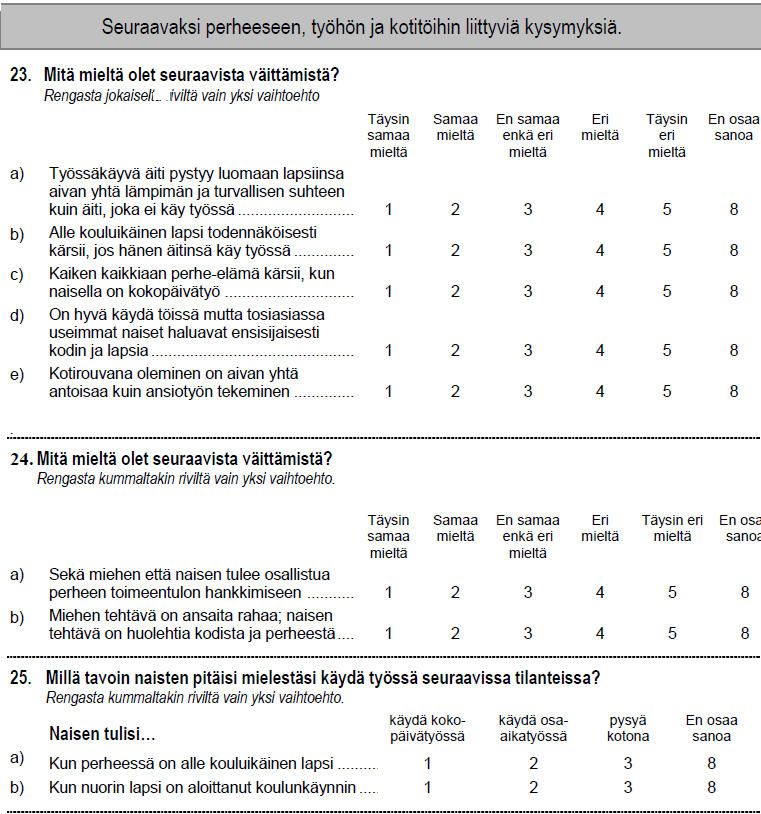
\includegraphics[width=0.5\linewidth]{img/substvar_fi_Q1Q2} 

}

\caption{Suomenkielinen lomake}\label{fig:suom-kys}
\end{figure}

\textbf{taustamuuttujat}

\textbf{k} maa, sukupuoli, haastateltavan ikä, koulutustaso, ``virallinen'' juridinen
parisuhdestatus, pääasiallinen toimi (töissä, eläkkeellä jne), lasten lukumäärä
perheessä ja asuinpaikka (maaseutu,suurkaupunki jne.), oma arvio sosiaalisesta
asemasta (1-10). Kysymyksiä, tiedot tosin kerätty eri tavoin eri maissa.

Vastaajan ikä

\textbf{K} Aineistossa mukana puuttuvat vastaukset, puuttuvia ei ole kolmessa muuttujassa
(maa, ikä ja sukupuoli). Muutamilla havainnoilla puuttui tieto iästä tai sukupuolesta,
ja ne rajattiin pois.

Kuvataan tarkemmin, kun käytetään luvussa 7.

\textbf{Miten aineistoa on käytetty?}.

\textbf{Korrespondenssianalyysin esimerkkiaineistona}

Michael Greenacre on käyttänyt aineistoa eri vuosilta luentomateriaaleissa (Helsinki 2017 MCA, viite Moodleen?) ja kahdessa oppikirjassa (\citep{RefWorks:doc:5a857a43e4b0ed2d44664d7c}, \citep{RefWorks:doc:5a857a43e4b0ed2d44664d78}).ISSP - aineisto vuodelta 1989 on käytetty myös neljän ``singuaariarvohajoitelmaan perustuvan menetelmän'' vertailuun\citep{RefWorks:doc:5b6f159ce4b0bc0f31734b76}.

``We consider the joint analysis of two matched matrices which have common
rows and columns, for example multivariate data observed at two time points or split
according to a dichotomous variable. Methods of interest include principal components
analysis for interval-scaled data, correspondence analysis for frequency data, log-ratio
analysis of compositional data and linear biplots in general, all of which depend on the
singular value decomposition. A simple result in matrix algebra shows that by setting up
two matched matrices in a particular block format, matrix sum and difference components
can be analysed using a single application of the singular value decomposition algorithm.
The methodology is applied to data from the International Social Survey Program
comparing male and female attitudes on working wives across eight countries. The resulting
biplots optimally display the overall cross-cultural differences as well as the male--female
differences. The case of more than two matched matrices is also discussed.''

Blasius ja Thiessen (\citep{RefWorks:doc:5b15542ee4b0e2616bc42dca}) arvioivat aineiston laatua ja ja maiden vertailtavuutta vuoden 1994 aineistolla.

``This paper provides empirically-based criteria for selecting Items and countries to develop measures of an underlying construct of interest that are comparable in cross-national research. Using data from the 1994 International Social Survey Program and applying multiple correspondence analysis to a set of common items in each of the 24 participating countries, we show that both the quality of the data, as well as its underlying structure - and therefore meaning - vary considerably between countries. The approach we use for screening countries and items is especially useful in situations where the psychometric properties of the items have not been well established in previous research.''

\textbf{tärkeä rajaus} Substanssitutkimusta ei tässä käsitellä.

``ISSP - saitilla'' löytyy bibliografia, ja hakupalveluillakin voi haravoida.
\textbf{zxy} www.gesis.org - sivustolta löytyy myös \href{https://search.gesis.org/research_data/ZA5900}{julkaisuluettelo}, voiko linkin laittaa alaviitteeksi tai suoraan leipätekstiin?

Sukupuoliroolien (gender roles) ja niihin liittyvien asenteiden vertailevaa kansainvälistä (cross-cultural) tutkimusta on tehty paljon. Tutkimusongelman sisällöllisten ja teoreettisen kysymysten nykytilaa kuvaa Walterin\citep{RefWorks:doc:5bd08fb6e4b05c5447c9a9f9} tuore artikkeli. Omnibus surveys ?

\hypertarget{yksinkertainen-korrespondenssianalyysi}{%
\chapter{Yksinkertainen korrespondenssianalyysi}\label{yksinkertainen-korrespondenssianalyysi}}

\textbf{k1} Yksi kysymys, kuusi maata, peruskäsitteet

\textbf{k2} Luvun tärkeimmät asiat; mitä on luvassa?

\hypertarget{uxe4iti-tuxf6issuxe4--kuxe4rsiikuxf6-lapsi}{%
\section{Äiti töissä -kärsiikö lapsi?}\label{uxe4iti-tuxf6issuxe4--kuxe4rsiikuxf6-lapsi}}

\textbf{k1}``Alle kouluikäinen lapsi todennäköisesti kärsii, jos hänen äitinsä käy työssä''.
Lyhennän muotoon äiti töissä. ISSP-tutkimuksissa kaksi kysymystä, joissa sana ``äiti'',
MG havainnut vastausten jakaumat poikkeaviksi (\textbf{\#V ?}).

\textbf{zxy} Edellisessä luvussa on esitelyt aineisto, ja kerrottu rajaukset.

Tarkistetaan uudet muuttujat (koodilohkon tulostus pois tarvittaessa).

\hypertarget{kahden-muuttujan-frekvenssitaulukon-analyysi}{%
\section{Kahden muuttujan frekvenssitaulukon analyysi}\label{kahden-muuttujan-frekvenssitaulukon-analyysi}}

\textbf{k} Kolme taulukkoa: frekvenssitaulukko, riviprosentit ja sarakeprosentit

\begin{table}

\caption{\label{tab:simpeCA-frekTa1}Kysymyksen Q1b vastaukset maittain, suhteelliset frekvenssit}
\centering
\begin{tabular}[t]{lllllll}
\toprule
  & S & s & ? & e & E & Total\\
\midrule
BE & 2.35 & 5.54 & 5.38 & 6.78 & 4.68 & 24.72\\
BG & 1.45 & 4.85 & 2.52 & 2.33 & 0.16 & 11.31\\
DE & 2.03 & 4.61 & 2.43 & 6.61 & 5.38 & 21.05\\
DK & 0.86 & 2.92 & 1.87 & 2.85 & 8.55 & 17.05\\
FI & 0.58 & 2.31 & 1.83 & 5.19 & 3.72 & 13.63\\
\addlinespace
HU & 2.69 & 3.54 & 2.76 & 2.33 & 0.92 & 12.24\\
Total & 9.95 & 23.76 & 16.79 & 26.10 & 23.41 & 100.00\\
\bottomrule
\end{tabular}
\end{table}

\begin{table}

\caption{\label{tab:simpeCA-rprosTa1}Kysymyksen Q1b vastaukset, riviprosentit}
\centering
\begin{tabular}[t]{lllllll}
\toprule
  & S & s & ? & e & E & Total\\
\midrule
BE & 9.49 & 22.40 & 21.76 & 27.42 & 18.93 & 100.00\\
BG & 12.81 & 42.89 & 22.26 & 20.63 & 1.41 & 100.00\\
DE & 9.63 & 21.88 & 11.55 & 31.39 & 25.55 & 100.00\\
DK & 5.04 & 17.15 & 10.95 & 16.71 & 50.14 & 100.00\\
FI & 4.23 & 16.94 & 13.42 & 38.11 & 27.30 & 100.00\\
\addlinespace
HU & 21.97 & 28.89 & 22.57 & 19.06 & 7.52 & 100.00\\
All & 9.95 & 23.76 & 16.79 & 26.10 & 23.41 & 100.00\\
\bottomrule
\end{tabular}
\end{table}

\begin{table}

\caption{\label{tab:simpeCA-cprosTa1}Kysymyksen Q1b vastaukset, sarakeprosentit}
\centering
\begin{tabular}[t]{lllllll}
\toprule
  & S & s & ? & e & E & All\\
\midrule
BE & 23.58 & 23.31 & 32.04 & 25.98 & 19.99 & 24.72\\
BG & 14.57 & 20.41 & 15.00 & 8.94 & 0.68 & 11.31\\
DE & 20.37 & 19.38 & 14.48 & 25.32 & 22.98 & 21.05\\
DK & 8.64 & 12.30 & 11.12 & 10.92 & 36.52 & 17.05\\
FI & 5.80 & 9.72 & 10.90 & 19.91 & 15.90 & 13.63\\
\addlinespace
HU & 27.04 & 14.88 & 16.46 & 8.94 & 3.93 & 12.24\\
Total & 100.00 & 100.00 & 100.00 & 100.00 & 100.00 & 100.00\\
\bottomrule
\end{tabular}
\end{table}

\textbf{k} \textbf{Taulkoista}

Frekvenssitaulukossa havaintojen lukumäärät on jaettu kokonaislukumäärällä
(8143).

Frekvenssitaulukko \ref{tab:simpeCA-frekTa1} kertoo vastausten jakauman maiden
ja vastausvaihtoehtojen mukaan luokiteltuina.

Muuttujien luonne on usein erilainen. Tähän aineistoon sopii riviprosenttientaulukko,
vertaillaan vastausten jakaumia maiden välillä.Taulukon sarakkeet ovat muuttujia
ja rivit havaintoja. Sarakeprosentit antavat toisen näkökulmaan samaan dataan.

\textbf{k} Rivit on saatu alkuperäisestä aineistosta osajoukkojen summina. MG:n
terminologialla ``samples''.

\textbf{Kuvat}

\begin{figure}
\centering
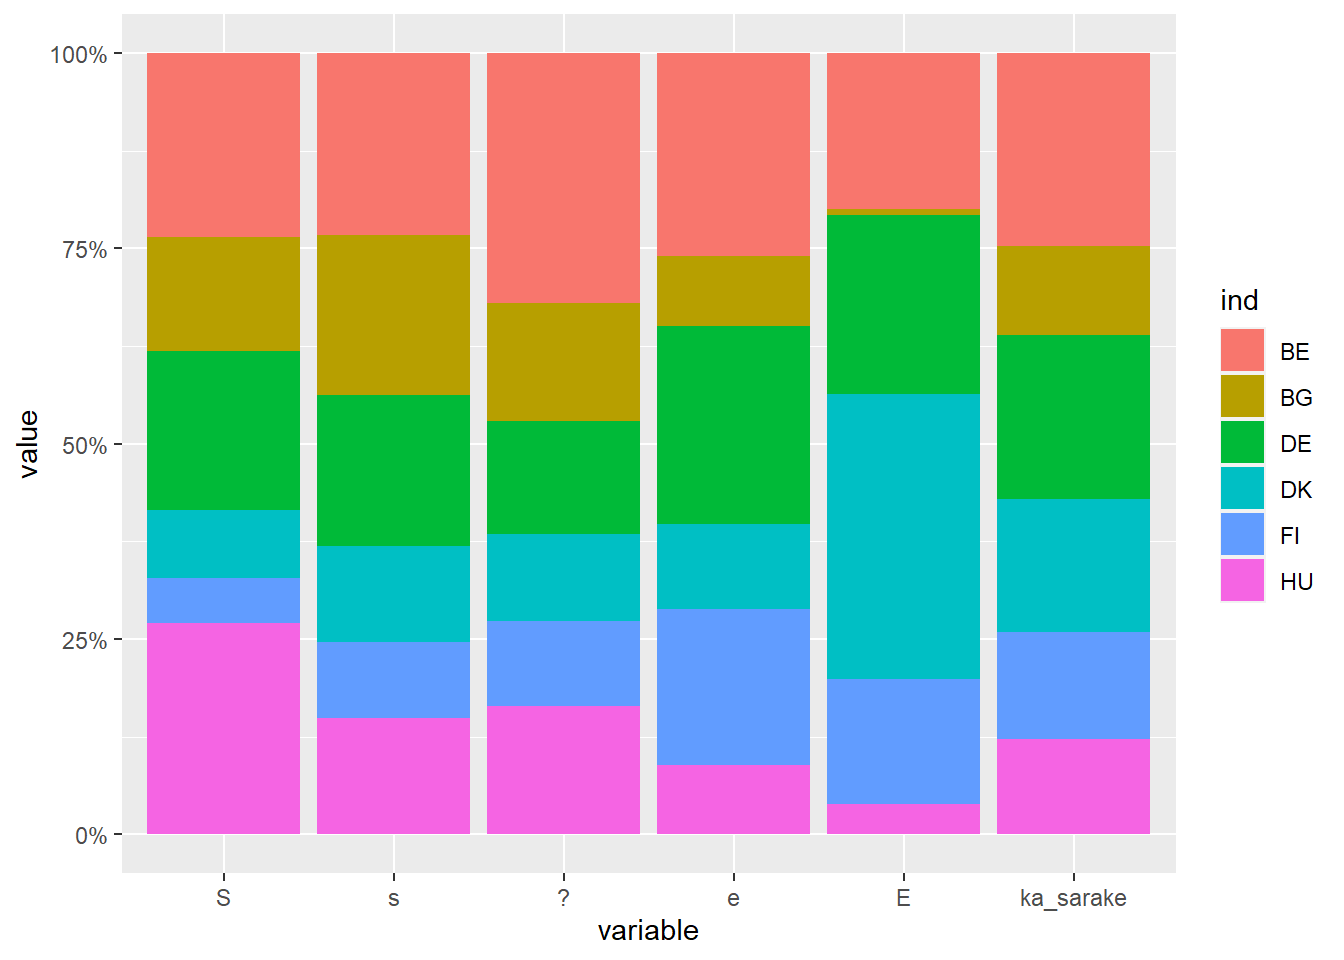
\includegraphics{JH_capaper_files/figure-latex/g1-2kuva1-1.pdf}
\caption{\label{fig:g1-2kuva1}Q1b:Sarakeprofiilit ja keskiarvoprofiili}
\end{figure}

\begin{figure}
\centering
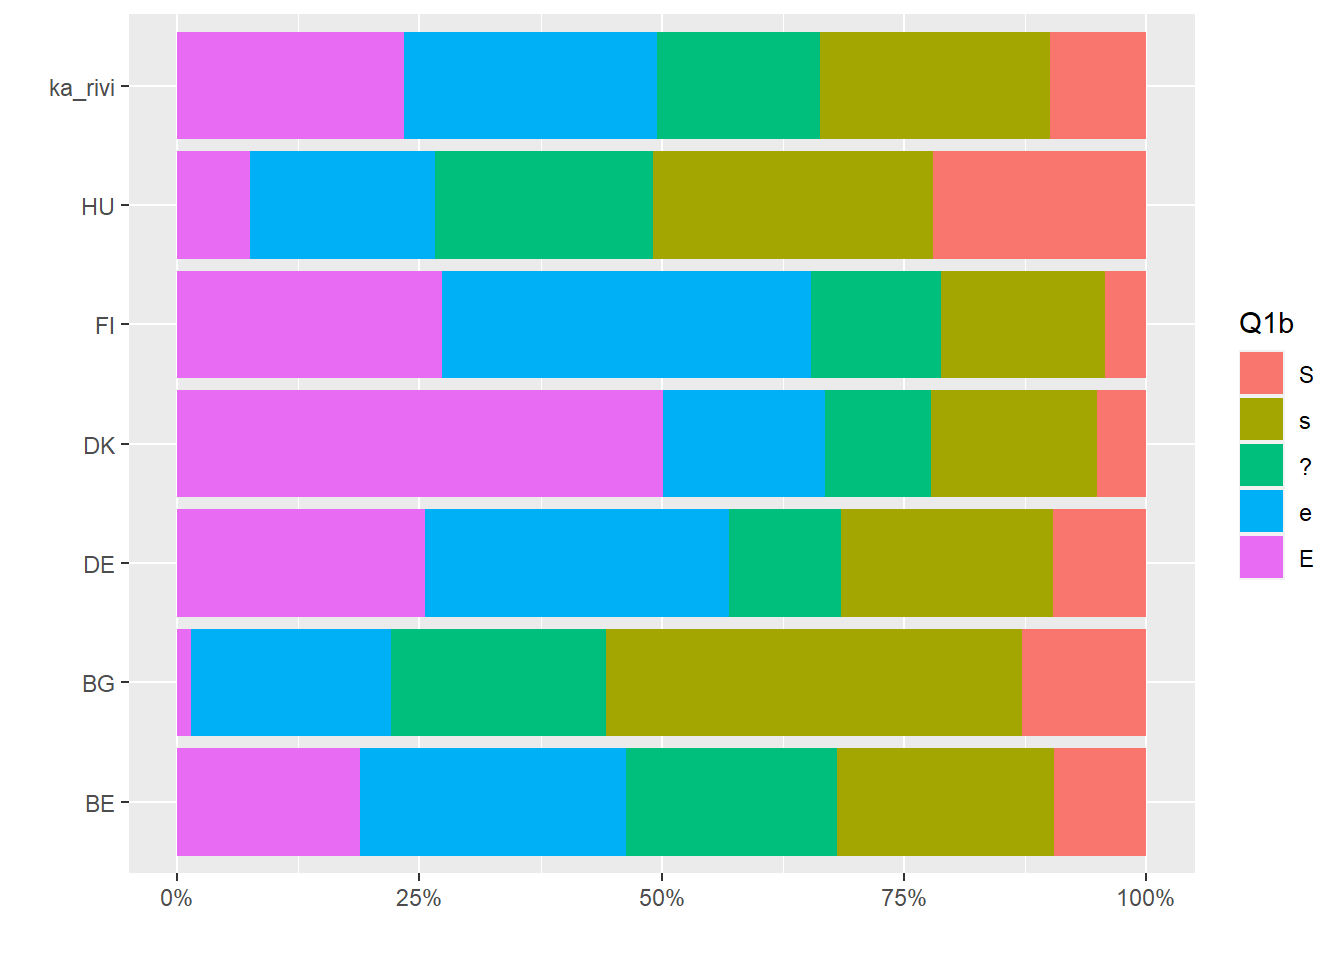
\includegraphics{JH_capaper_files/figure-latex/g1-2kuva2-1.pdf}
\caption{\label{fig:g1-2kuva2}Q1b: riviprofiilit ja keskiarvorivi}
\end{figure}

Mikä on rivien ja sarakkeiden suhde?

Tähän klassiseen kysymykseen korrespondenssianalyysi tarjoaa oman ratkaisunsa.
Siinä rivit ja sarakkeet esitetään samassa kuvassa, ja riippuutta tutkitaan tulkitsemalla tämä kuva tai ``kartta''.

Kahden luokittelumuuttujan riippuvuutta voidaan testata \(\chi^{2}\) - testillä.
Testisuure saadaan laskemalla yhten jokaisen solun havaittujen ja odotetettujen
(riippumattomuushypoteesi) frekvenssien erotukset muodossa

\begin{equation}
  \chi^{2} = \frac{(havaittu - odotettu)^2} {odotettu}
    \label{eq:khii21}
\end{equation}

Tämä voidaan esittää ca:han sopivammalla tavalla parilla muunnoksella, jolloin
saamme riveittäin vastaavat termit rivisummalla painotettuna:

\begin{equation}
  rivisumma \times \frac{(havaittu \: riviprofiili - odotettu \: riviprofiili)^2} {odotettu \: riviprofiili}
    \label{eq:khii22}
\end{equation}

Kun jaamme nämä tekijät havaintojen kokonaismäärällä \(n\), rivisumma muuntuu
rivin massaksi, ja niiden summa muotoon \(\frac{\chi^{2}}{n}\).

\begin{equation}
 \frac{\chi^{2}}{n} = \phi^{2}
  \label{eq:inert1}
 \end{equation}

Huomaa jakajassa n, ei n-1. Tässä ei tn-päättelyä!

Tunnusluku \(\phi^{2}\) on korrespondenssianalyysissä kokonaisinertia (total
inertia). Se kuvaa, kuinka paljon varianssia taulukossa on ja on riippumaton
havaintojen lukumäärästä. Tilastotieteessä tunnusluvulla on useita vaihtoehtoisia
nimiä (esim. mean square contingency coefficient), ja sen neliöjuurta kutsutaan
\(\phi\) - kertoimeksi.

Tässä siirrytään kahden luokittelumuuttujan taulukosta suhteellisten frekvenssien
taulukkoon. Kaavojen \eqref{eq:khii21} ja \eqref{eq:khii22} yhteyden pitäisi olla
selkeä.

Frekvenssitaulukossa (jossa kaikki taulukon luvut on jaettu havaintojen
lukumäärällä N riviprofiilien 1 ja 3 (euklidinen) etäisyys on

\begin{equation}
 \sqrt{(p_{11} - p_{31})^2 + (p_{12} - p_{32})^2 + (p_{13} - _{33})^2+ (p_{14} - _{34})^2+ (p_{15} - _{35})^2}
 \label{eq:euclid1}
 \end{equation}

Rivien \(\chi^{2}\) - etäisyys on painotettu euklidinen etäisyys, jossa painoina
ovat riviprofiilin odotetut arvot. Ne ovat riippumattomuushypoteesin mukaisesti
riviprofiilien keskiarvoprofiilin vastaavat alkioit \(r_{i}\) .

\begin{equation}
 \sqrt{\frac{(p_{11} - p_{31})^2} { r_{1}} + \dots + \frac{(p_{15} - p_{35})^2} {r_{5}}}
 \label{eq:euclid2}
\end{equation}

Inertia voidaa esittää rivien ja keskiarvorivin (sentroidin) \(\chi^{2}\) -etäisyyksien
neliöiden painotettuna summana, jossa painoina ovat rivien massat \(m_{i}\) ja
summa lasketaan yli rivien \({i}\).

\begin{equation}
 \phi^{2} = \sum_{i} (massa \: m_{i}) \times (profiilin \: i \: \chi^{2} - etaisyys \: sentroidista)^{2}
 \label{eq:inert2}
\end{equation}

Tässä esitystavassa viite on CAiP, teorialiitteessä tarkemmin. Tarkoitus on esittää
yksinkertaisesti taulukon datan analyysin käsitteet ja CA:n peruskäsitteet profiili,
massa ja \(\chi^{2}\) - etäisyys

\hypertarget{ca---esimerkki}{%
\section{CA - esimerkki}\label{ca---esimerkki}}

\begin{figure}

{\centering 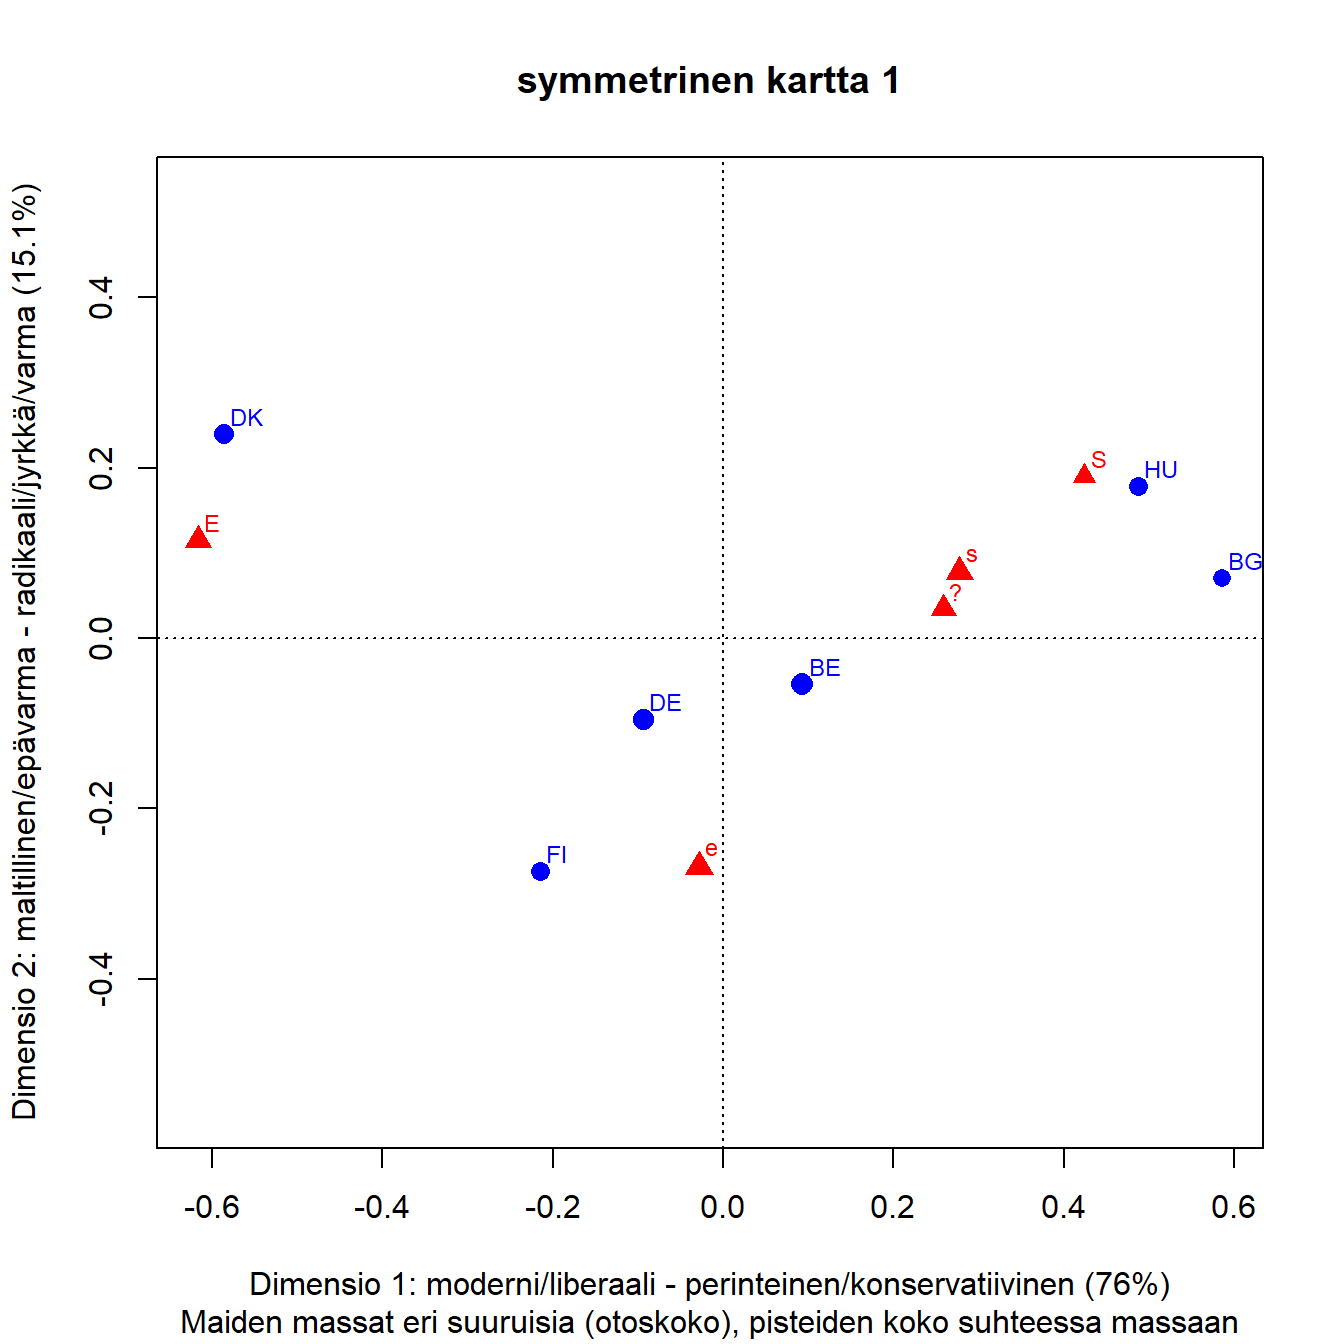
\includegraphics[width=0.9\linewidth]{JH_capaper_files/figure-latex/simpleCA1map1-1} 

}

\caption{Q1b: lapsi kärsii jos äiti on töissä}\label{fig:simpleCA1map1}
\end{figure}

\textbf{edit1} jatkossa plot - main on kuvan tyyppi (symmetrinen, kontribuutio jne),
koodilohkon fig.cap ``ylimmän tason'' otsikko.

\textbf{edit2} Akseleiden tekstit (Dimensio 1\ldots.jne) asetettu käsin, ikävä kyllä myös
selitetyn inertian osuus. Ainakin tästä ensimmäisestä kuvasta ne kannattaa jättää
pois, spoileri!

\textbf{edit3} par(cex = 1) ennen plot-komenota muuttaa valitettavasti ``kaiken'' kokoa.
Antaa olla, kun on graafista data-analyysiä. Selkeys tärkeämpää kuin ulkoasu.

\textbf{k} Kartan tulkinta

\textbf{k} Prosentit - kuinka paljon kokonaisinertiasta saadaan kuvattua (``selitettyä'').

\textbf{k} Dimenisoiden tulkinta sarakepisteiden avulla: mitä on oikealla ja vasemmalla?
Kaukana on kaukana, mutta lähellä voi olla täydessä sarake- tai riviavaruudessa
kaukana. Siksi tulkinta kontrastien avulla - mikä piste on suhteellisesti kauimpana?

\textbf{k} Rivipisteiden tulkinta kartalla - järjestys vasemmalta oikealle ja alhaalta
ylös. Pisteiden etäisyydet toisistaan.

\textbf{k} Origo on aineiston keskipiste, ``riippumattomuushypoteesi'' (kts. teorialiite).

\textbf{k} Sarakepisteiden erot ja rivipisteiden erot ovat suhteellisia, approksimoivat
khii2-etäisyyksiä.

\textbf{k} Rivi- ja sarakepisteiden etäisyyksillä ei suoraan mitään tulkintaa!

\textbf{k} Lista: mitä muuta, johon palataan seuraavassa luvussa?

\begin{itemize}
\tightlist
\item
  kuinka hyvin pisteet on esitetty tasossa?
\item
  esim. x-akseli kuvaa (``nappaa'') 76\% kokonaisinertiasta. Pisteiden
  inertiakontribuutiot
\end{itemize}

\hypertarget{korrespondenssianalyysin-peruskuxe4sitteet}{%
\section{Korrespondenssianalyysin peruskäsitteet}\label{korrespondenssianalyysin-peruskuxe4sitteet}}

\textbf{ks} Mitä käsitteitä tässä esitellään? Viittaukset teorialiitteeseen, ja
tulkinnan hankaluudet (MG ``loose ends'' - paperi) käsitellään siellä.

\textbf{edit} Sulava kuvaus tulkinnasta, painotus kuvien tulkinnassa. CA:n numeeriset
tulokset vasta seuraavassa luvussa. Tässä ``mitä kuvasta näkee'', ei muuta (paitsi
varoitukset - mitä ei näe). Idea koko ajan taulukon sarakkeiden ja riveien yhteyksien
visualisointi.

\textbf{edit} Tärkeää selkeä kuvaus pääkoordinaattien ja standardikoordinaattien
suhteesta. Tarkemmin teorialiitteessä, tässä heuristisesti jotta kuvia osaa tulkita.

\hypertarget{asymmetrinen-kartta-ja-ideaalipisteet}{%
\subsection{Asymmetrinen kartta ja ideaalipisteet}\label{asymmetrinen-kartta-ja-ideaalipisteet}}

\begin{figure}

{\centering 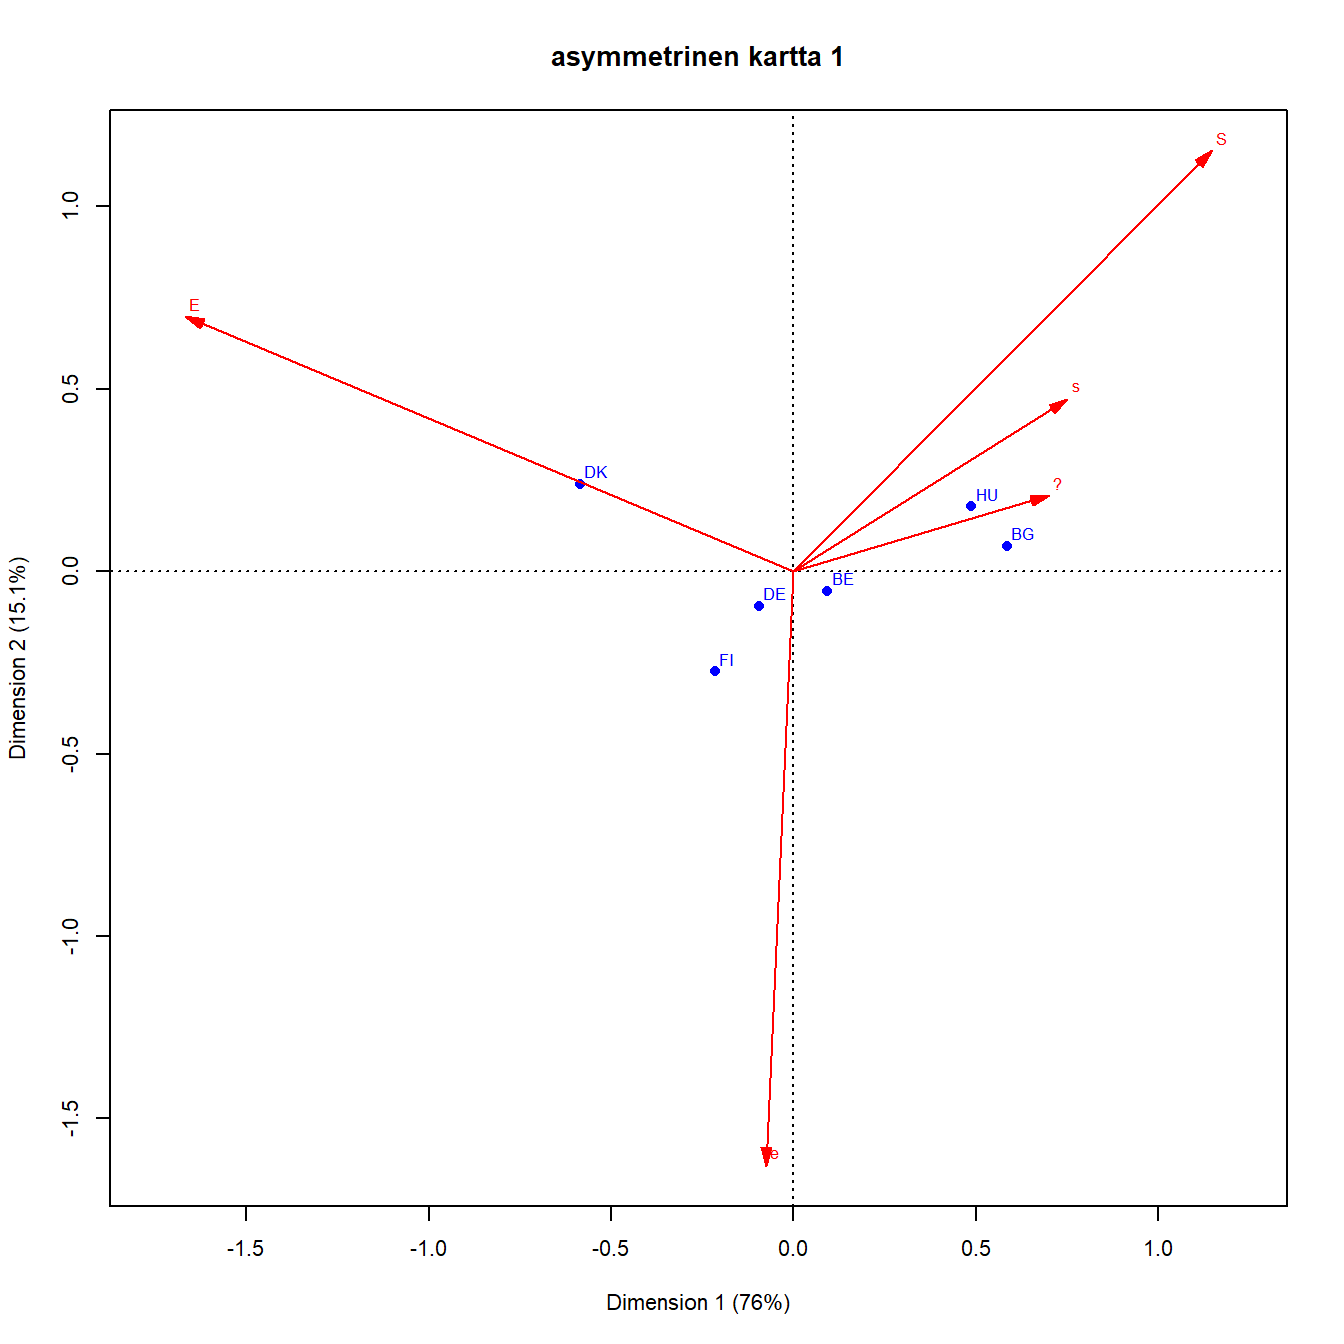
\includegraphics[width=0.9\linewidth]{JH_capaper_files/figure-latex/G1-3asymm2-1} 

}

\caption{Q1b: lapsi kärsii jos äiti on töissä}\label{fig:G1-3asymm2}
\end{figure}

\textbf{Barysentrinen periaate}

\textbf{edit} kuva ei ehkä tarpeen? Tehdään vähän pienempi (out.width = 70\%, muuten 90\%).

\begin{figure}

{\centering 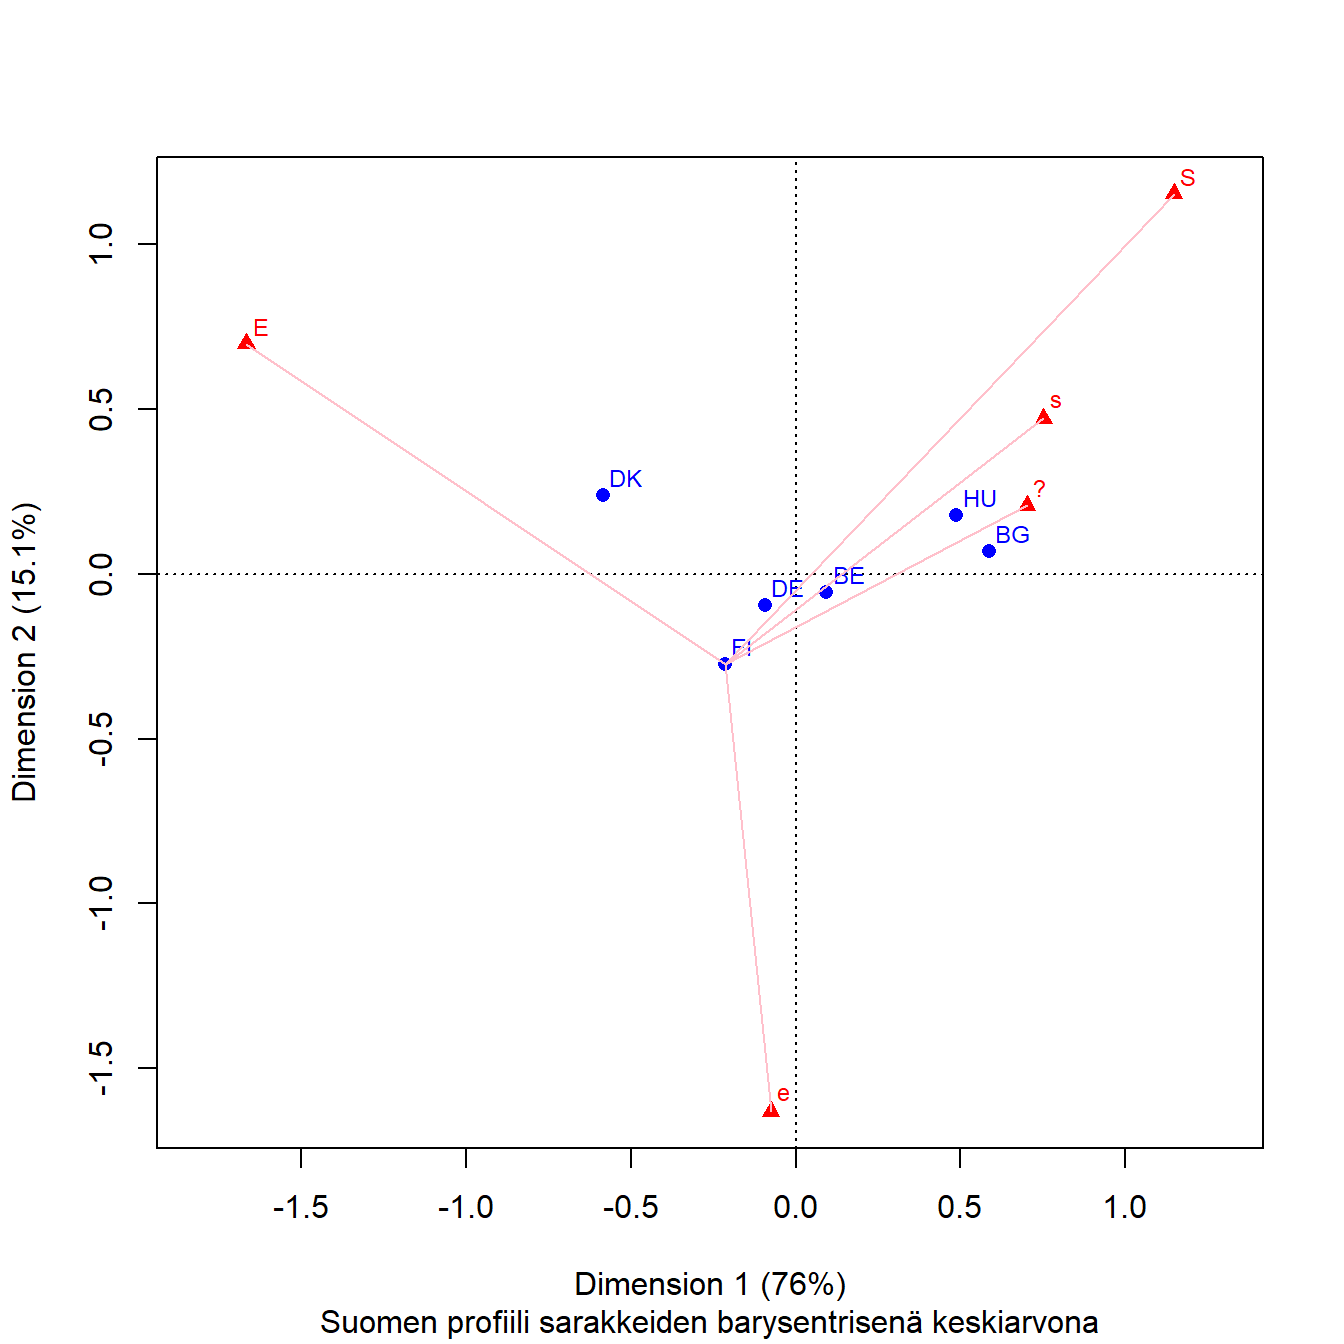
\includegraphics[width=0.7\linewidth]{JH_capaper_files/figure-latex/G1-3asymm3-1} 

}

\caption{Q1b: lapsi kärsii jos äiti on töissä}\label{fig:G1-3asymm3}
\end{figure}

\textbf{edit} Perustelu kuvalle: barysentrinen periaate on kuvien tulkinnassa ydinasioita.

\textbf{Akseleiden tulkinta} tai tulkinnan varmistaminen akseli kerrallaan. Ortogonaaliset
projektion piirretty käsin, havainnollistetaan periaatetta.

\begin{center}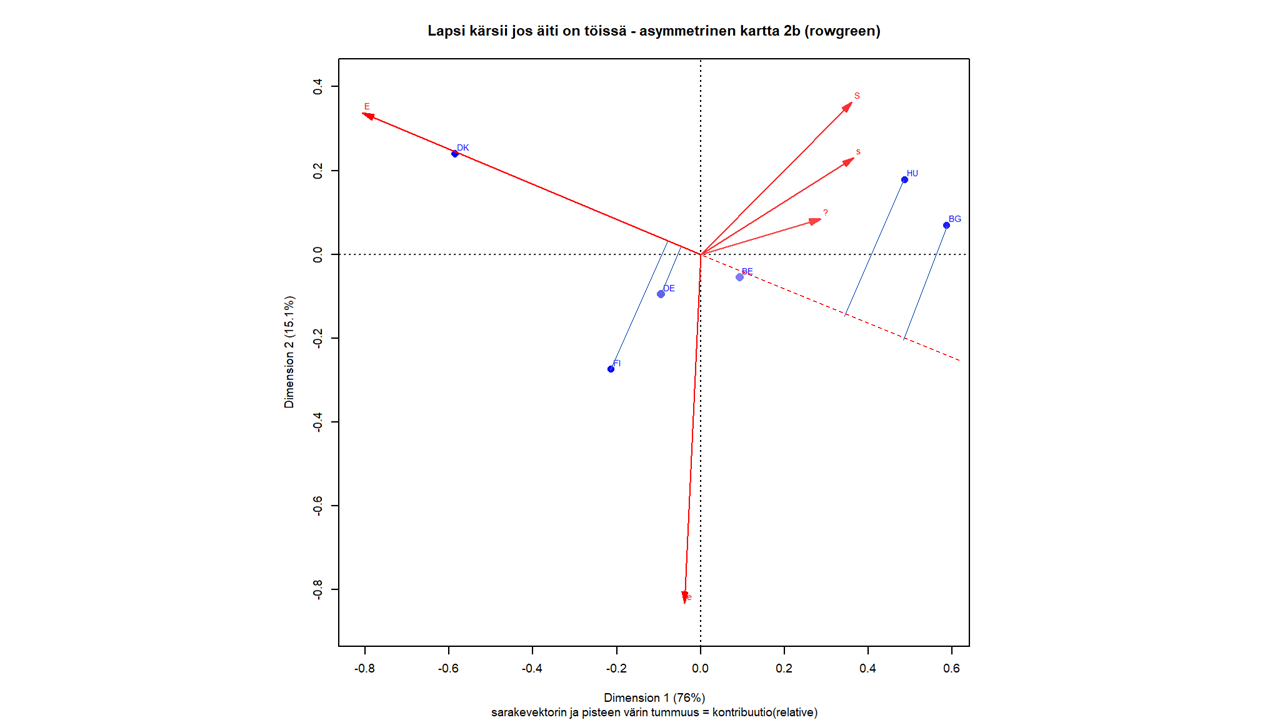
\includegraphics[width=0.9\linewidth]{img/simpleCAasymmTulk2} \end{center}

\hypertarget{kontribuutiot-kartalla}{%
\section{Kontribuutiot kartalla}\label{kontribuutiot-kartalla}}

Kaksi kuvaa, joissa pisteiden massat on kuvattu pisteiden koolla (ei juuri eroa
huomaa) ja rivi- ja sarekepisteiden kontribuutiot värisävyllä. Mitä tummempi sitä
suurempi kontribuutio. Absoluuttiset ja suhteelliset kontribuutiot.

\textbf{edit} Pitäisikö kuvissa olla aina toinen absolute, toinen relative? Selvitetään
teorialiittessä?

Toinen kuva riittää, tässä esitellään kartta jossa on eniten informaatiota.

\textbf{Absoluuttiset kontribuutiot} Oletuspistekoko ok, mutta html- ja pdf-tulostus
on erilainen!

\begin{figure}

{\centering 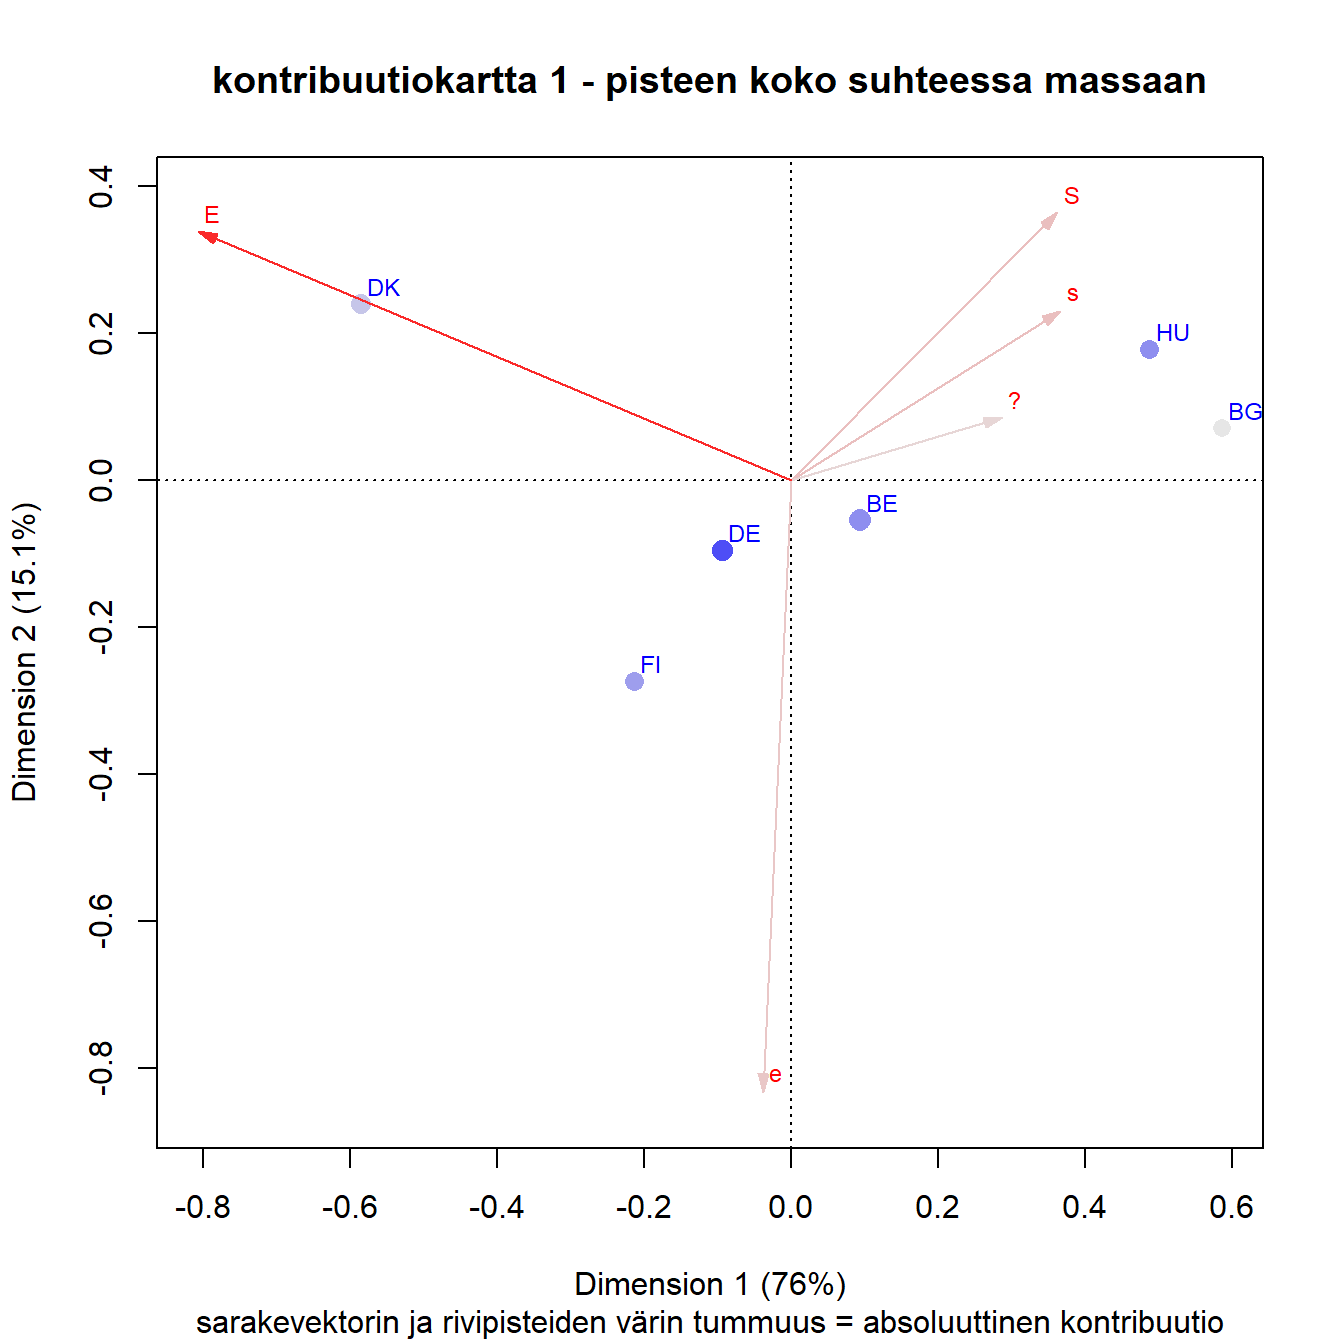
\includegraphics[width=0.9\linewidth]{JH_capaper_files/figure-latex/G1-3asymmContrib1-1} 

}

\caption{Q1b: lapsi kärsii jos äiti on töissä}\label{fig:G1-3asymmContrib1}
\end{figure}

\textbf{Suhteelliset kontribuutiot} Oletuspistekoko ok.

\begin{figure}

{\centering 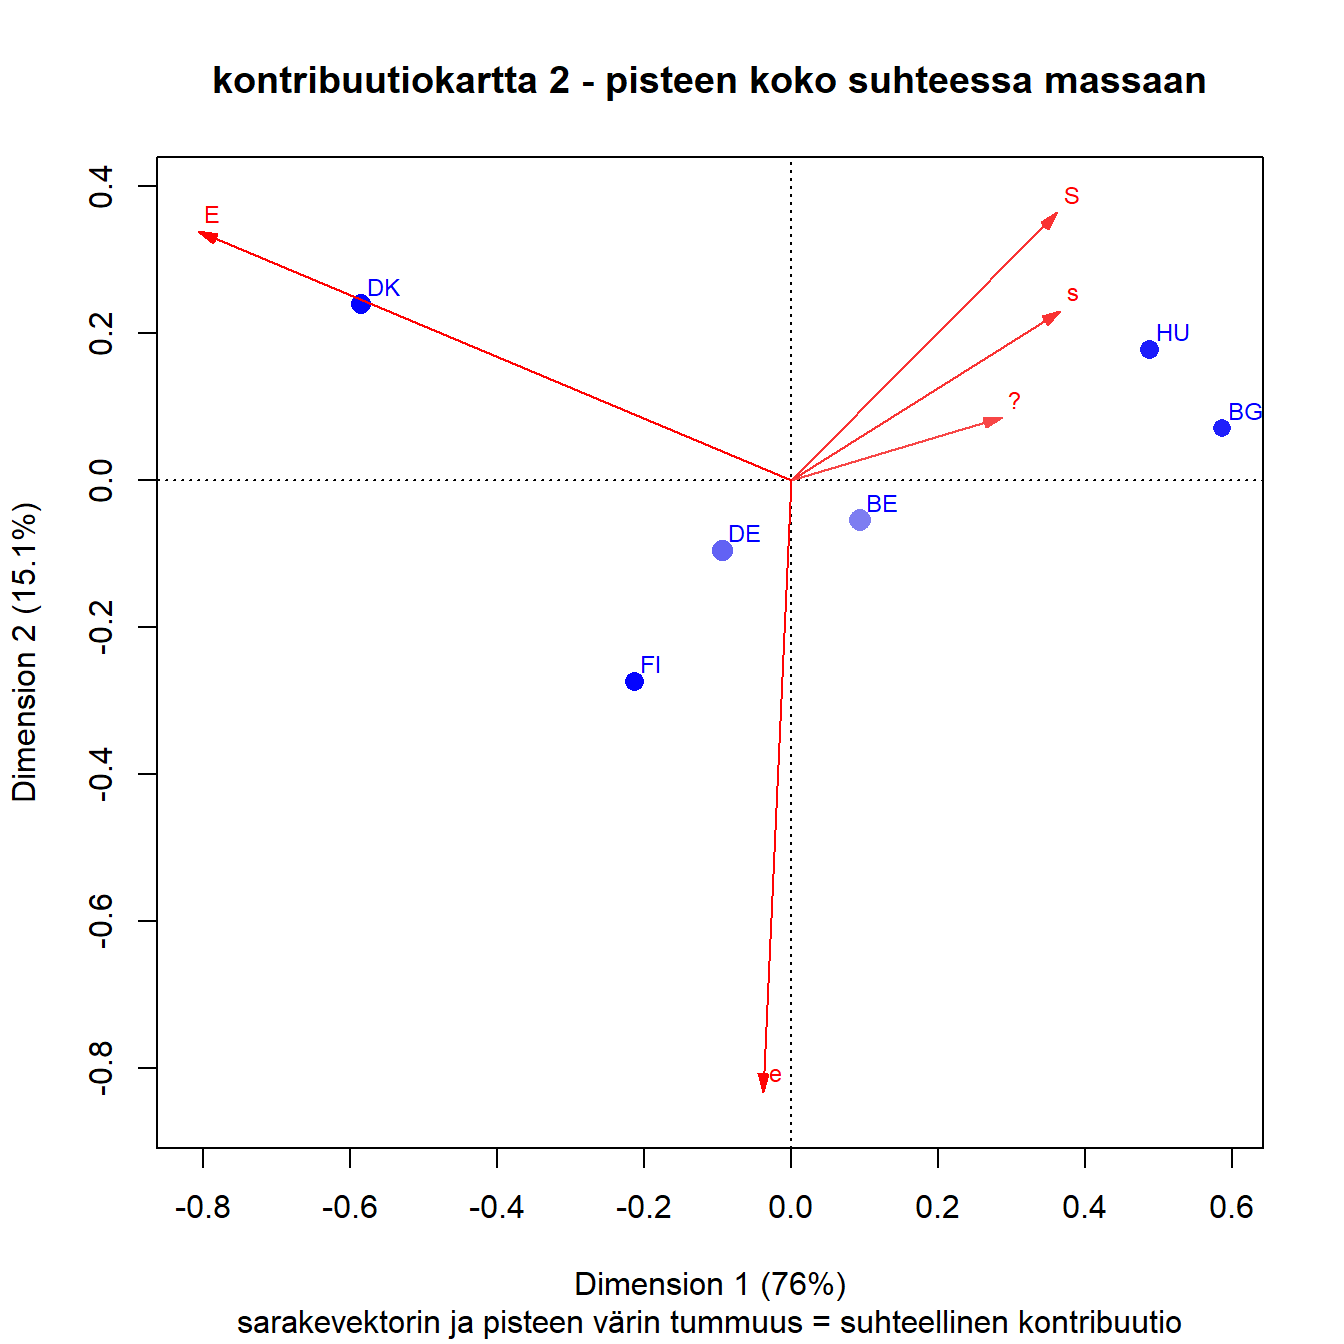
\includegraphics[width=0.9\linewidth]{JH_capaper_files/figure-latex/G1-3asymmContrib2-1} 

}

\caption{Q1b: lapsi kärsii jos äiti on töissä}\label{fig:G1-3asymmContrib2}
\end{figure}

\hypertarget{massat}{%
\section{Massat}\label{massat}}

\textbf{edit3} Onko vakioitujen massojen kartta liian aikaisin? Tämä ei ole pääasia, vaan selvennys.
Miksi tässä? Perusteltava, miksi en vakioi massoja maille, sukupuolille jne. (a)
perusteltua kun tarkempi tutkimusongelma, esim. erottelut maiden ja sukupuolten
välillä. Varianssianalyysin tapaan varianssin hajoittaminen ryhmisen sisäiseen ja
ryhmien väliseen. Kts. teorialiitteestä esim. ABBA. (b) CA ``perusmuodossa'', massa
on yksi kolmesta tärkeimmästä käsitteestä. (c) on aika työlästä!

\textbf{edit4} Galkussa verrattu molempien painotusten khii2-etäisyyksiä, jos tarpeen
niin teoria-liitteeseen.

\begin{figure}

{\centering 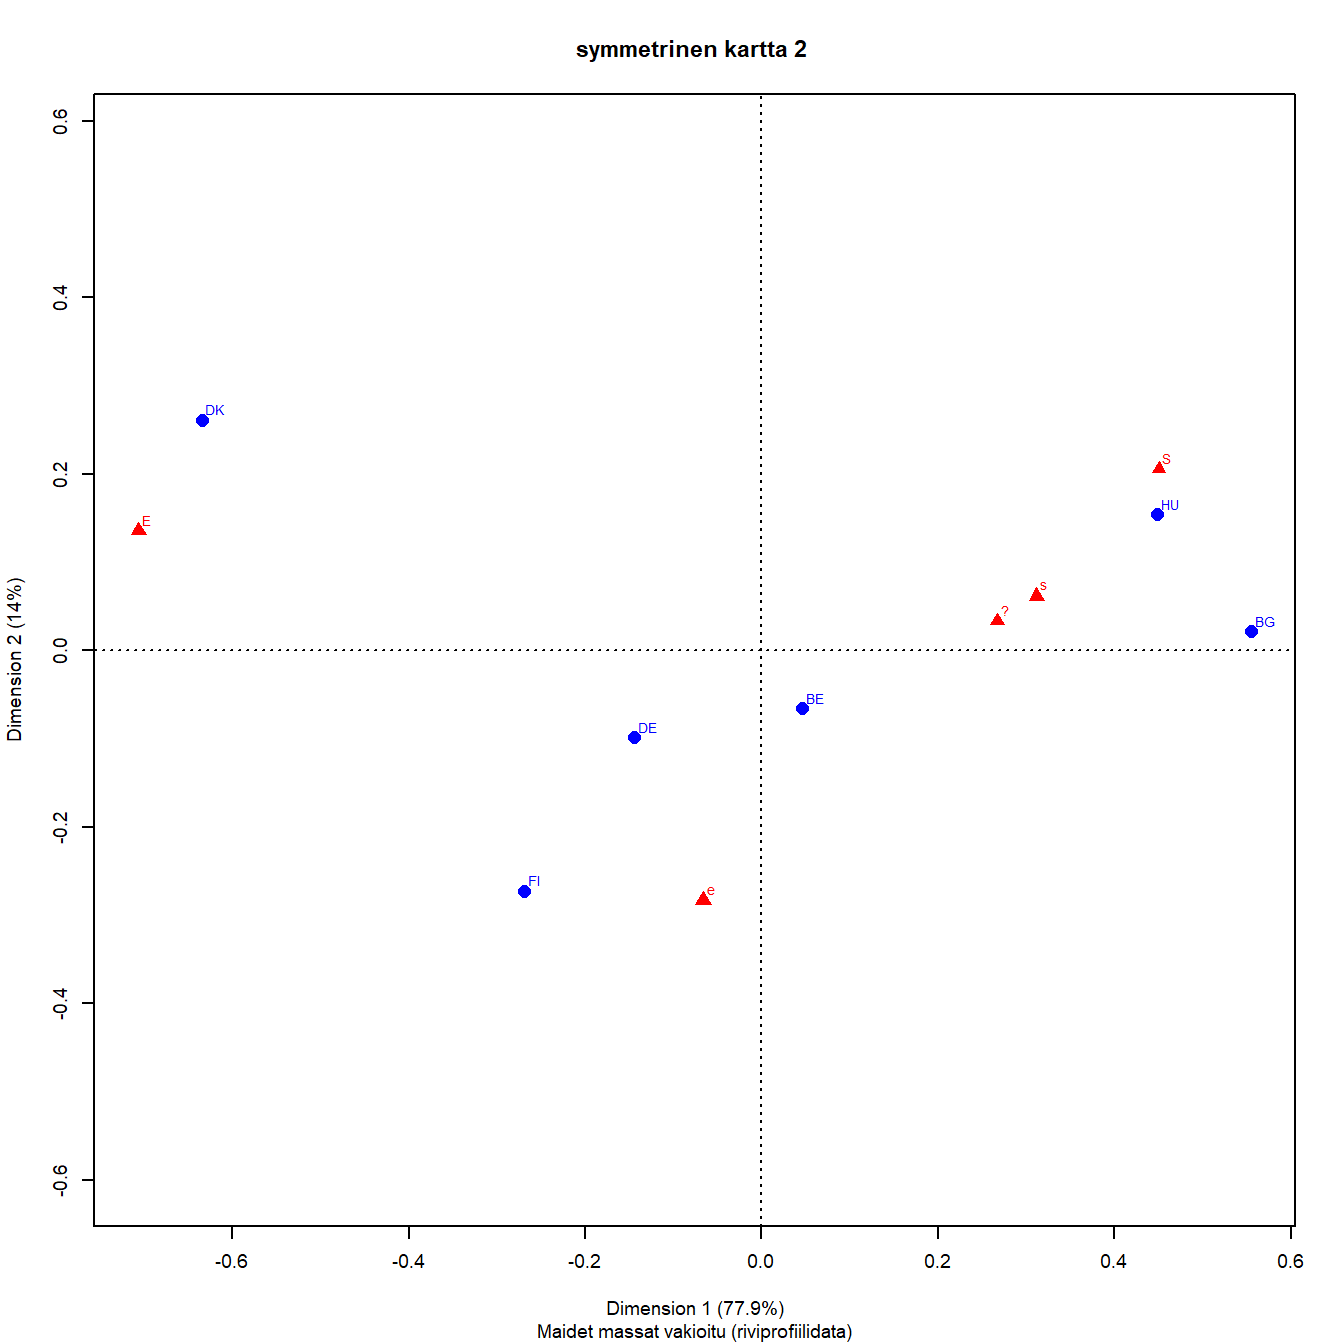
\includegraphics[width=0.9\linewidth]{JH_capaper_files/figure-latex/simpleCA3map1-1} 

}

\caption{Q1b: lapsi kärsii jos äiti on töissä}\label{fig:simpleCA3map1}
\end{figure}

Ei kovin isoja eroja, tässä datassa.

\hypertarget{yksinkertaisen-korrespondenssianalyysin-laajennuksia-1---tuxe4ydentuxe4vuxe4t-pisteet}{%
\chapter{Yksinkertaisen korrespondenssianalyysin laajennuksia 1 - täydentävät pisteet}\label{yksinkertaisen-korrespondenssianalyysin-laajennuksia-1---tuxe4ydentuxe4vuxe4t-pisteet}}

\textbf{edit} Edellisssä luvussa selitetty barysentrinen keskiarvopiste;
teorialiitteessä hieman laveammin.

\textbf{edit} CA:n joustava käyttö vaatii matriisioperaatioita, ja muuta datan rakenteen
muokkausta (rivien lisääminen input-dataan jne.).

\hypertarget{tuxe4ydentuxe4vuxe4t-pisteet-supplementary-points}{%
\section{Täydentävät pisteet (supplementary points)}\label{tuxe4ydentuxe4vuxe4t-pisteet-supplementary-points}}

Tekstistä oma dokkari, eri käyttötapaukset lyhyesti. Edellisen luvun asymmetrisen
kartan avulla perustellaan, miten pisteitä voidaaan lisätä.

\hypertarget{saksan-ja-belgian-alueet}{%
\section{Saksan ja Belgian alueet}\label{saksan-ja-belgian-alueet}}

\textbf{Data ja taulukko aluejaosta}

\begin{Shaded}
\begin{Highlighting}[]
\CommentTok{# riviprofiilitaulukko aiheuttaa virheen PDF-tulostuksessa, JH_capaper.Rmd}
\CommentTok{# tiedoston voi kuitenkin renderöidä knit-napilla RStudiossa pdf-tiedostoksi.}

\CommentTok{# Kts. edellinen koodilohko - testailua pdf-ongelman ratkaisemiseksi}
\CommentTok{# tallennetaan data tiedostoon, koodilohko BeDeAluedat1 passiviseksi}
\CommentTok{# suppoint1_tab1 <- read_rds("suppoint1tab1.rds")}
\CommentTok{# suppoint1_tab1 # tarkistus ok}

\CommentTok{# BeDealueTable <- ISSP2012esim1.dat %>% tableX(maa3, Q1b, type = "row_perc")}

\CommentTok{# knitr::kable(BeDealueTable , digits = 2, booktabs = TRUE,}
\CommentTok{#            caption = "Q1b vastaukset, Saksan ja Belgian alueet")}

\CommentTok{# Q1b vastaukset, Saksan ja Belgian alueet}
\CommentTok{# S s   ?   e   E   Total}
\CommentTok{# bF    5.04    23.81   25.89   30.83   14.43   100.00}
\CommentTok{# bW    10.82   21.02   18.57   24.08   25.51   100.00}
\CommentTok{# bB    17.03   20.94   16.63   23.87   21.53   100.00}
\CommentTok{# BG    12.81   42.89   22.26   20.63   1.41    100.00}
\CommentTok{# dW    11.40   26.82   11.83   32.13   17.82   100.00}
\CommentTok{# dE    5.85    11.33   10.97   29.80   42.05   100.00}
\CommentTok{# DK    5.04    17.15   10.95   16.71   50.14   100.00}
\CommentTok{# FI    4.23    16.94   13.42   38.11   27.30   100.00}
\CommentTok{# HU    21.97   28.89   22.57   19.06   7.52    100.00}
\CommentTok{# All   9.95    23.76   16.79   26.10   23.41   100.00}
\end{Highlighting}
\end{Shaded}

Taulukko, Saksan ja Belgian alueet ja maaprofiilit.

\textbf{edit} Riviprofiilitaulukko, kuvataan alueiden eroja. CA-analyysi kuitenkin koko
aineiston frekfvenssitaululla, jossa rivien massat eivät ole samat.

\hypertarget{symmetrinen-kartta}{%
\subsection{Symmetrinen kartta}\label{symmetrinen-kartta}}

\begin{figure}

{\centering 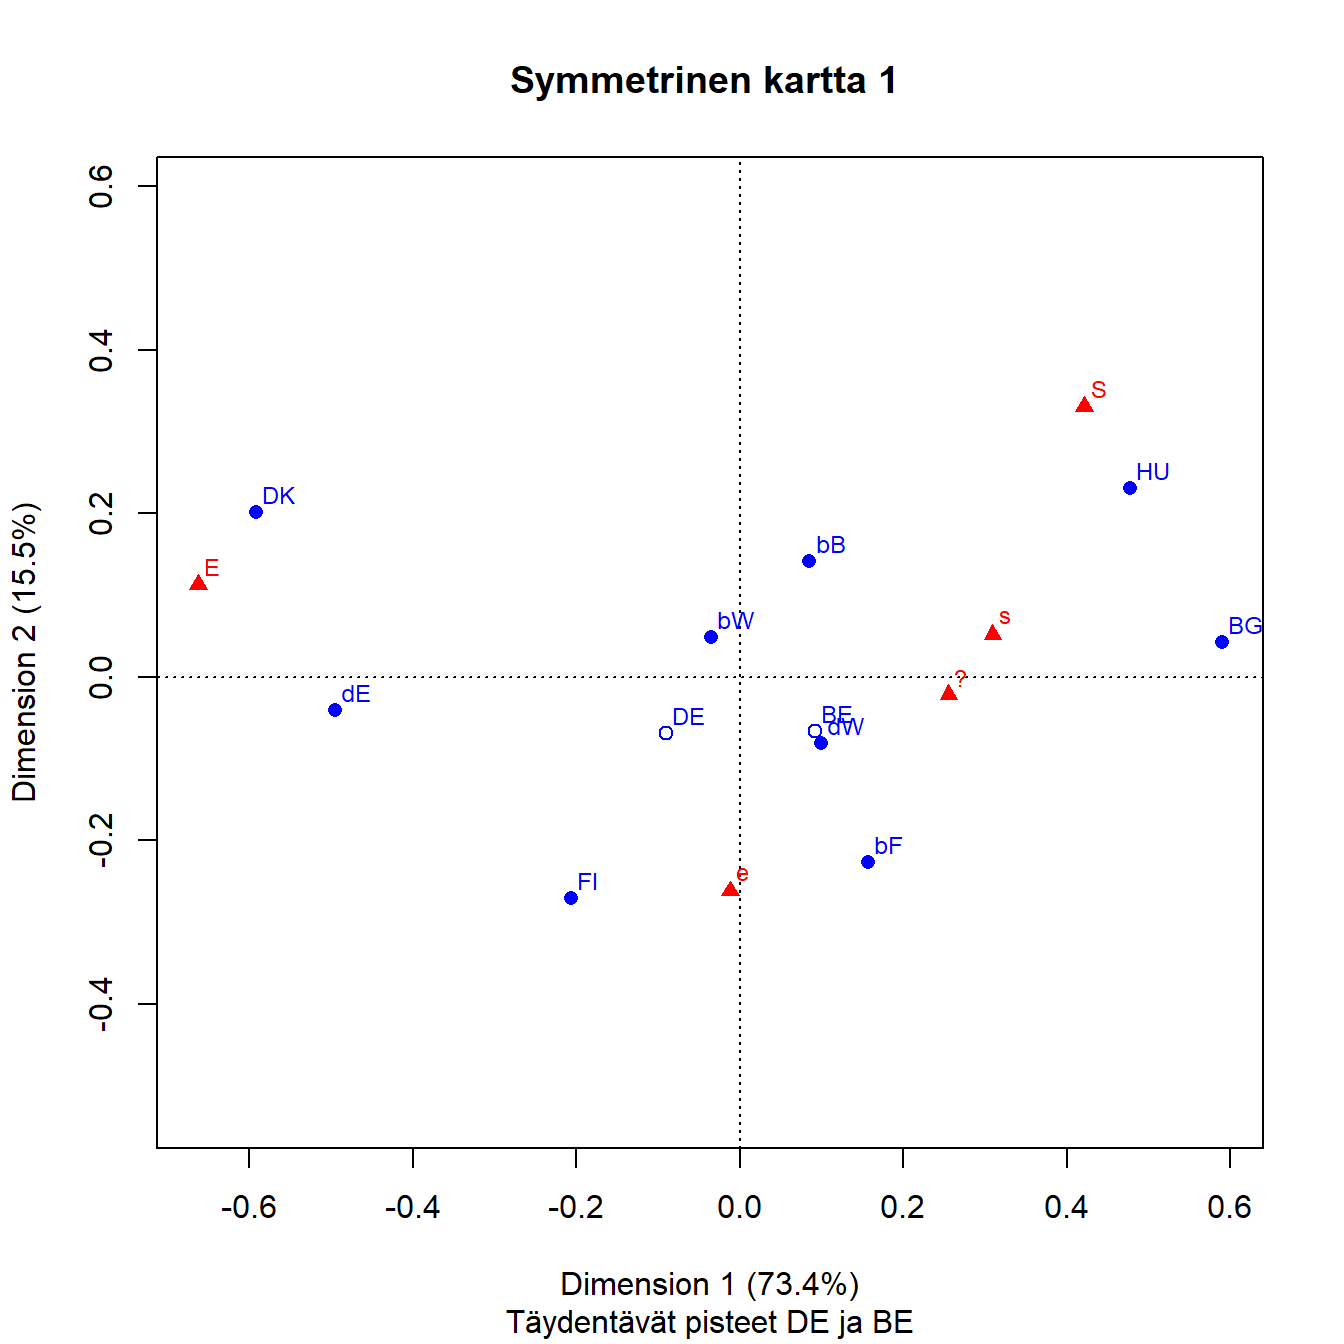
\includegraphics[width=0.9\linewidth]{JH_capaper_files/figure-latex/suppointCA2map1-1} 

}

\caption{Q1b: Saksan ja  Belgian aluejako }\label{fig:suppointCA2map1}
\end{figure}

\textbf{k} Maaåpisteet alueiden barysentrinen keskiarvo. Tulkinta.

\begin{figure}

{\centering 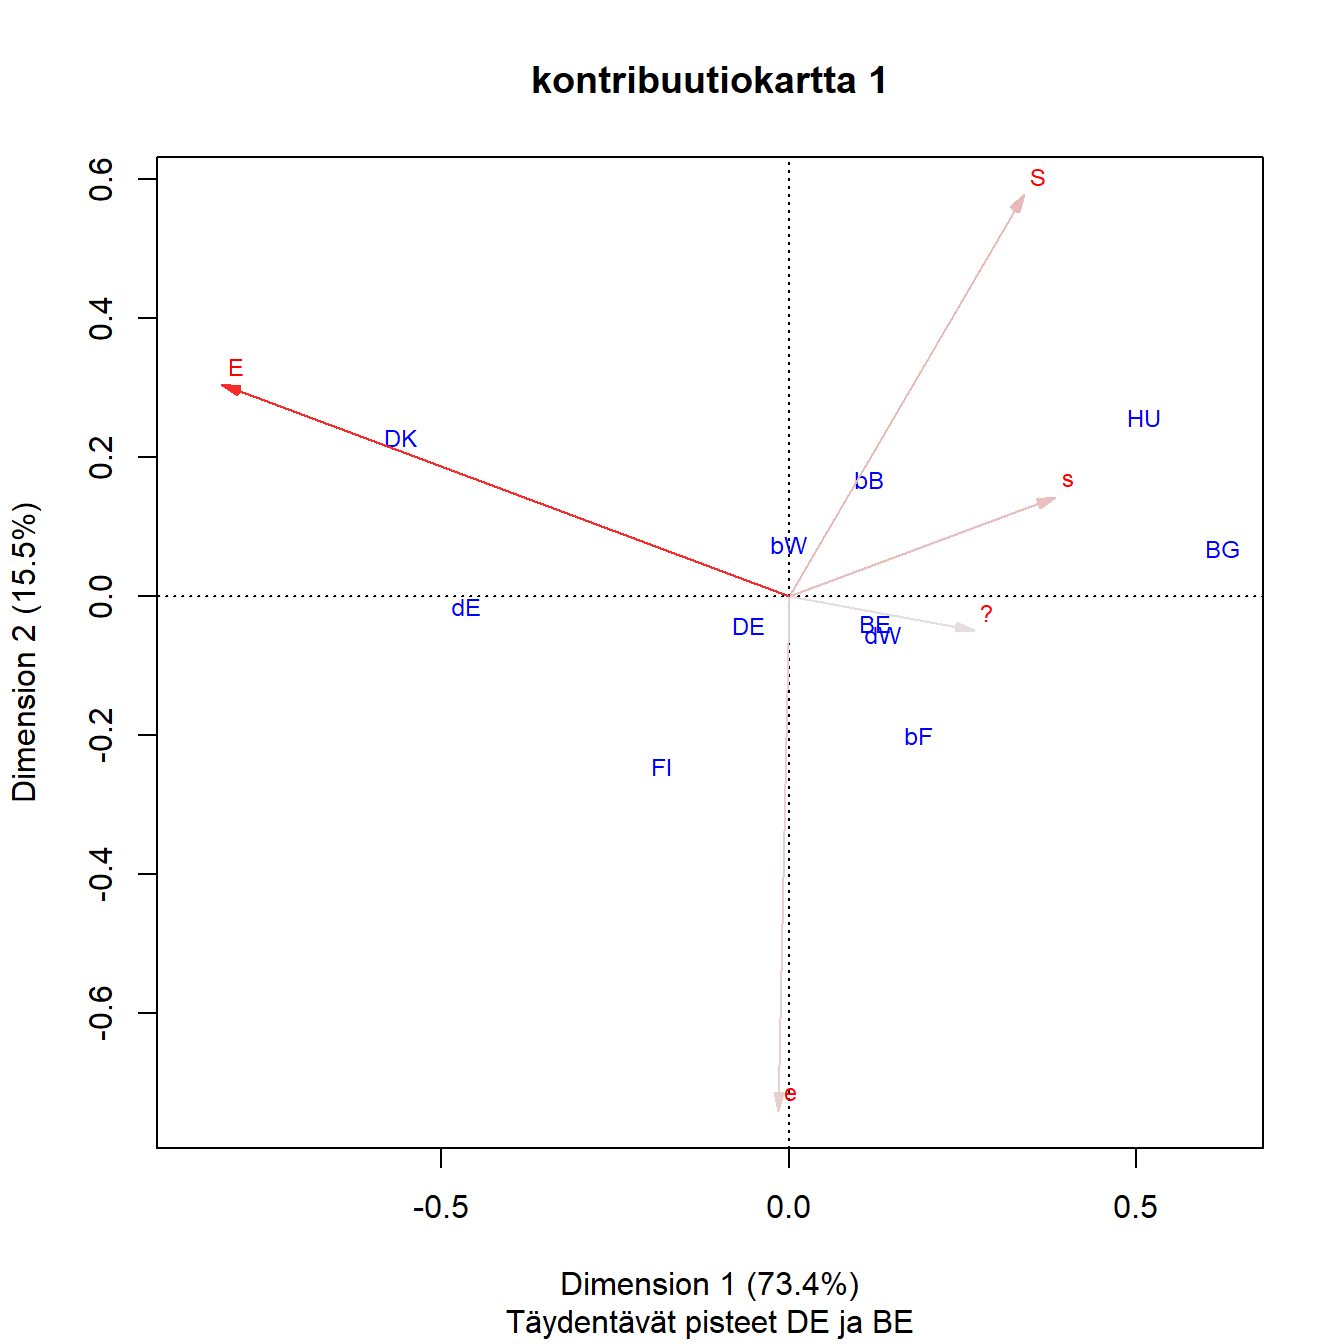
\includegraphics[width=0.9\linewidth]{JH_capaper_files/figure-latex/suppointCA2map2-1} 

}

\caption{Q1b: Saksan ja  Belgian aluejako }\label{fig:suppointCA2map2}
\end{figure}

\textbf{k} Kontribuutiokartta, kontribuutio värisävyinä ja massat pisteiden kokona.
Yleiskuvaan riittävä, ei kovin selkeä yksityiskohdissa. Motivaatio seuraavalle
jaksolle.Skaalataan asymmetrisen kuvan sarakevektoreita (jotka standardikoordinaateissa)
hieman lähemmäs origoa.

\textbf{k} Kaukana on kaukana, mutta lähellä voi olla myös kaukana.

\hypertarget{can-numeeriset-tulokset}{%
\section{CA:n numeeriset tulokset}\label{can-numeeriset-tulokset}}

\textbf{edit} Teorialiitteessä selitetään tarkemmin numeeristen tulosten tausta, tässä
apuneuvo (a) kuvan tulkinnan varmistamiseen ja (b) approksimaation laadun
tarkistamiseen.

\begin{Shaded}
\begin{Highlighting}[]
\NormalTok{suppointCA2}
\end{Highlighting}
\end{Shaded}

\begin{verbatim}
## 
##  Principal inertias (eigenvalues):
##            1        2        3        4       
## Value      0.154101 0.032489 0.014294 0.008944
## Percentage 73.44%   15.48%   6.81%    4.26%   
## 
## 
##  Rows:
##                bF        bW       bB       BG        dW        dE        DK
## Mass     0.124279  0.060174 0.062753 0.113103  0.143313  0.067174  0.170453
## ChiDist  0.341469  0.096258 0.239034 0.630991  0.219094  0.505720  0.634063
## Inertia  0.014491  0.000558 0.003586 0.045032  0.006879  0.017180  0.068528
## Dim. 1   0.400065 -0.090631 0.216912 1.502458  0.254323 -1.262007 -1.506022
## Dim. 2  -1.254042  0.267998 0.789358 0.236498 -0.451124 -0.226595  1.121468
##                FI       HU    BE (*)    DE (*)
## Mass     0.136313 0.122436        NA        NA
## ChiDist  0.347733 0.550404  0.157974  0.175013
## Inertia  0.016483 0.037091        NA        NA
## Dim. 1  -0.525222 1.215462  0.234127 -0.229593
## Dim. 2  -1.500986 1.280342 -0.364834 -0.379468
## 
## 
##  Columns:
##                S        s         ?         e         E
## Mass    0.099472 0.237627  0.167874  0.260960  0.234066
## ChiDist 0.592824 0.354761  0.332288  0.280549  0.672594
## Inertia 0.034959 0.029907  0.018536  0.020540  0.105887
## Dim. 1  1.073310 0.787257  0.649789 -0.029859 -1.688108
## Dim. 2  1.835133 0.290929 -0.119934 -1.451548  0.629110
\end{verbatim}

\textbf{k} Lyhyt selostus - nämä aika selkeitä

\begin{Shaded}
\begin{Highlighting}[]
\KeywordTok{summary}\NormalTok{(suppointCA2)}
\end{Highlighting}
\end{Shaded}

\begin{verbatim}
## 
## Principal inertias (eigenvalues):
## 
##  dim    value      %   cum%   scree plot               
##  1      0.154101  73.4  73.4  ******************       
##  2      0.032489  15.5  88.9  ****                     
##  3      0.014294   6.8  95.7  **                       
##  4      0.008944   4.3 100.0  *                        
##         -------- -----                                 
##  Total: 0.209828 100.0                                 
## 
## 
## Rows:
##       name   mass  qlt  inr    k=1 cor  ctr    k=2 cor  ctr  
## 1  |    bF |  124  650   69 |  157 212   20 | -226 438  195 |
## 2  |    bW |   60  388    3 |  -36 137    0 |   48 252    4 |
## 3  |    bB |   63  481   17 |   85 127    3 |  142 354   39 |
## 4  |    BG |  113  878  215 |  590 874  255 |   43   5    6 |
## 5  |    dW |  143  345   33 |  100 208    9 |  -81 138   29 |
## 6  |    dE |   67  966   82 | -495 960  107 |  -41   7    3 |
## 7  |    DK |  170  971  327 | -591 869  387 |  202 102  214 |
## 8  |    FI |  136  957   79 | -206 352   38 | -271 605  307 |
## 9  |    HU |  122  927  177 |  477 751  181 |  231 176  201 |
## 10 | (*)BE | <NA>  512 <NA> |   92 338 <NA> |  -66 173 <NA> |
## 11 | (*)DE | <NA>  418 <NA> |  -90 265 <NA> |  -68 153 <NA> |
## 
## Columns:
##     name   mass  qlt  inr    k=1 cor ctr    k=2 cor ctr  
## 1 |    S |   99  816  167 |  421 505 115 |  331 311 335 |
## 2 |    s |  238  781  143 |  309 759 147 |   52  22  20 |
## 3 |      |  168  594   88 |  255 589  71 |  -22   4   2 |
## 4 |    e |  261  871   98 |  -12   2   0 | -262 870 550 |
## 5 |    E |  234  999  505 | -663 971 667 |  113  28  93 |
\end{verbatim}

\textbf{k} Tulosteen käsitteiden esittely - tavoite kuvan laadun varmistus, akselien
tulkinnan tarkistus. Tarkemmin teorialiitteessä. Tästä pitäisi nähdä, miksi seuraavat
kartat ovat sellaisia kuin ovat.

\hypertarget{esimerkki-3d--kartasta---saksan-ja-belgian-dimensiot}{%
\section{Esimerkki 3d- kartasta - Saksan ja Belgian dimensiot}\label{esimerkki-3d--kartasta---saksan-ja-belgian-dimensiot}}

\textbf{k} Ei kovin hyviä kuvia, mutta periaate on tärkeä. Kartta on approksimaatio,
pitää päättää milloin se on tarpeeksi hyvä. Tai mille pisteille hyvä, mille huonompi.

\textbf{edit 26.10.2020} summary-funktio ei toimi, kun dimensioita CA-ratkaisussa kolme.
Numeeriset tulokset voisi laskea ``käsityönä''. Kehno kvalitetti 2d-ratkaisussa saa
kuvissa selityksen.

\begin{Shaded}
\begin{Highlighting}[]
\NormalTok{suppointCA3 <-}\StringTok{ }\KeywordTok{ca}\NormalTok{(}\OperatorTok{~}\NormalTok{maa3 }\OperatorTok{+}\StringTok{ }\NormalTok{Q1b,ISSP2012esim1.dat, }\DataTypeTok{nd =} \DecValTok{3}\NormalTok{)}

\CommentTok{# summary(suppointCA3)}
\CommentTok{# Error in rsc %*% diag(sv) : non-conformable arguments}
\end{Highlighting}
\end{Shaded}

\textbf{Kolme karttaa}

\begin{figure}

{\centering 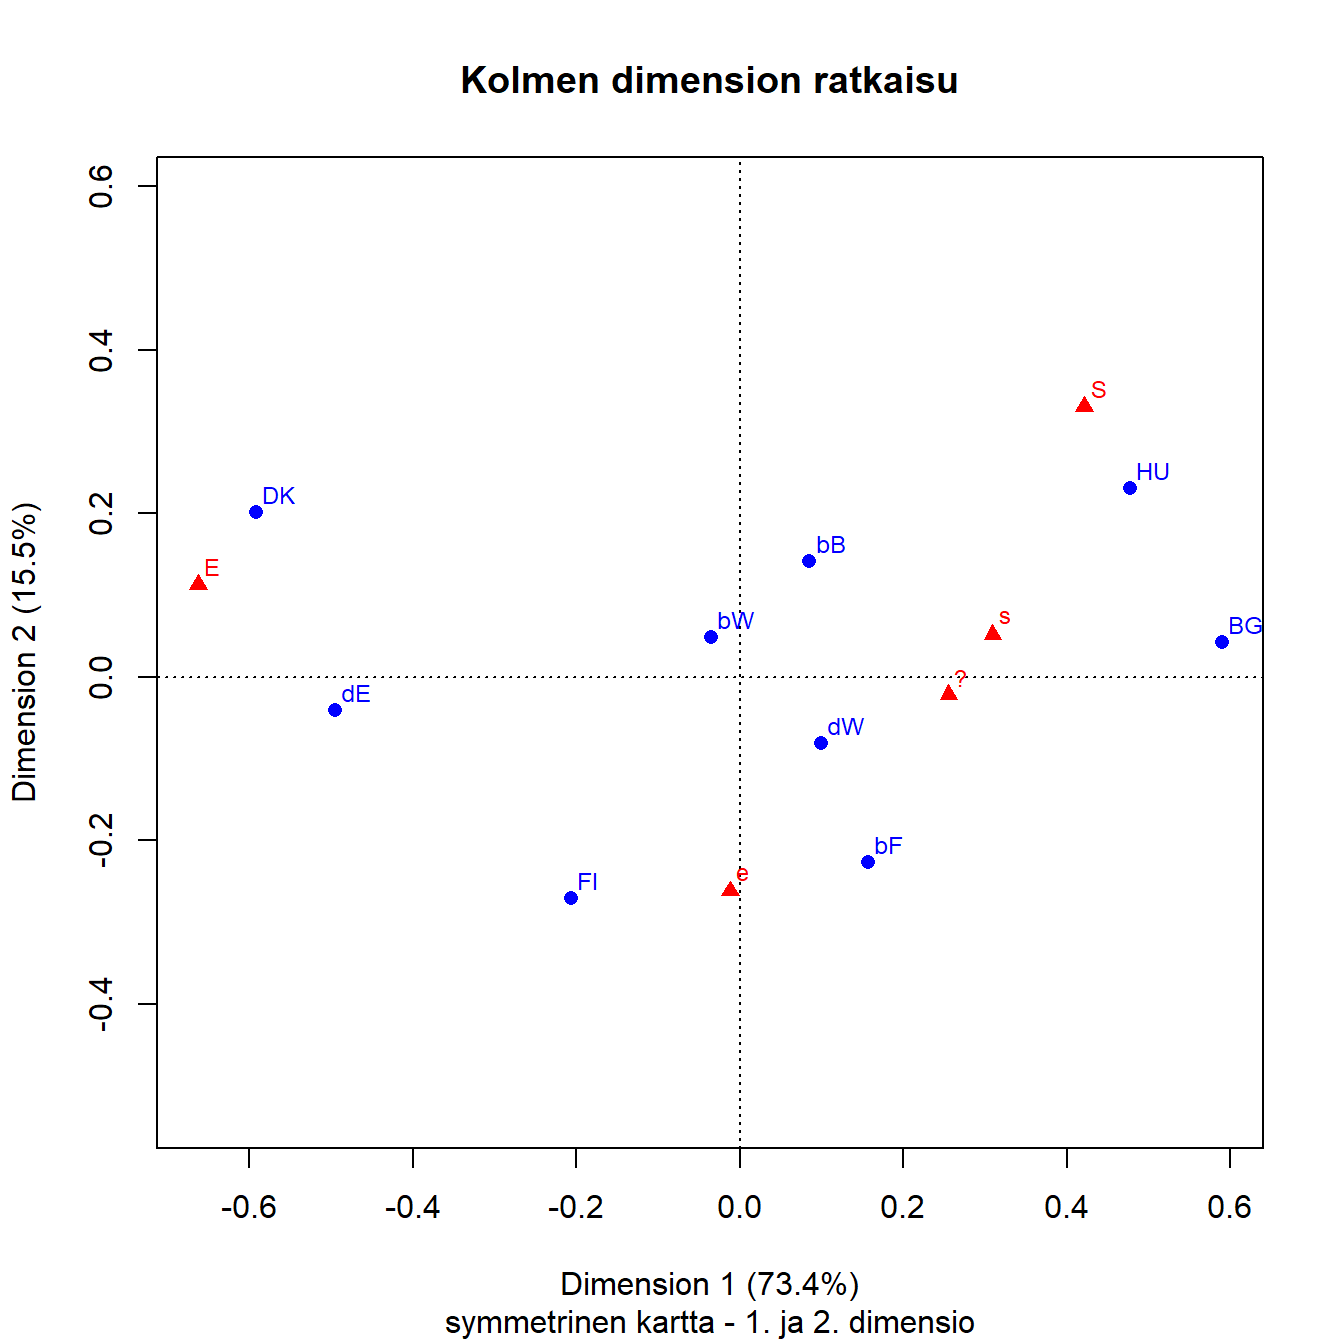
\includegraphics[width=0.9\linewidth]{JH_capaper_files/figure-latex/suppointCA3map1-1} 

}

\caption{Q1b: Saksan ja  Belgian aluejako }\label{fig:suppointCA3map1}
\end{figure}

\begin{figure}

{\centering 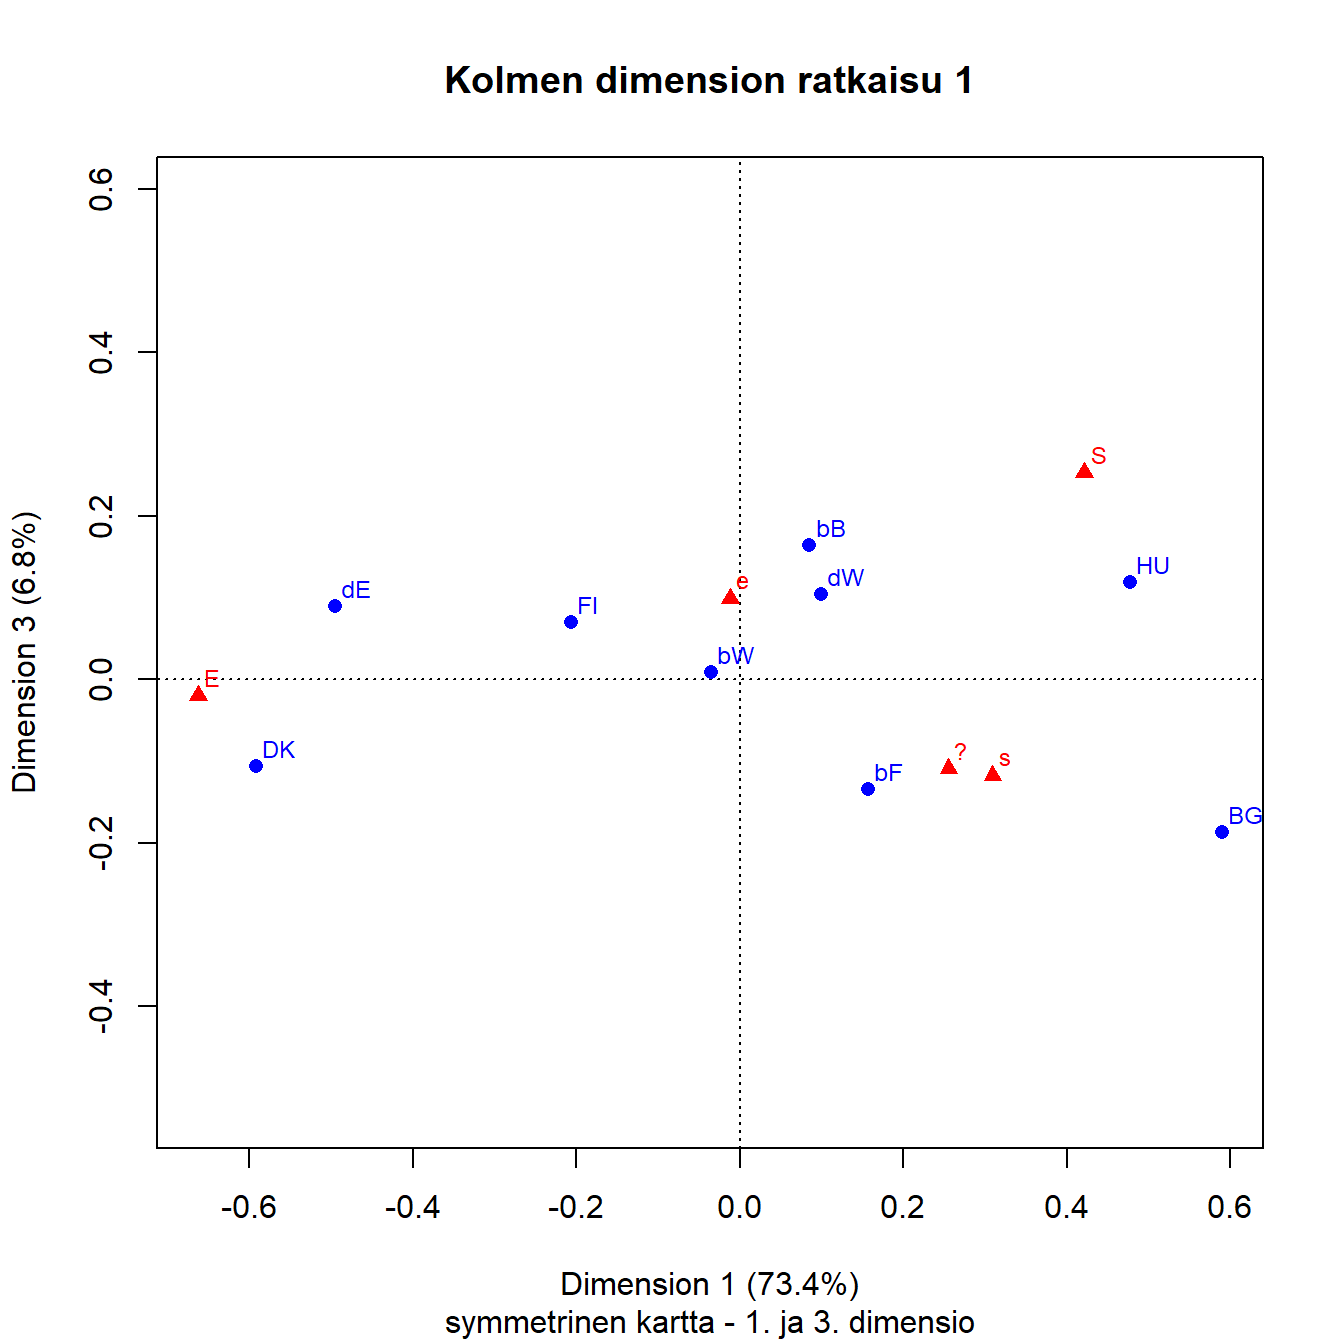
\includegraphics[width=0.9\linewidth]{JH_capaper_files/figure-latex/suppointCA3map2-1} 

}

\caption{Q1b: Saksan ja  Belgian aluejako }\label{fig:suppointCA3map2}
\end{figure}

\begin{figure}

{\centering 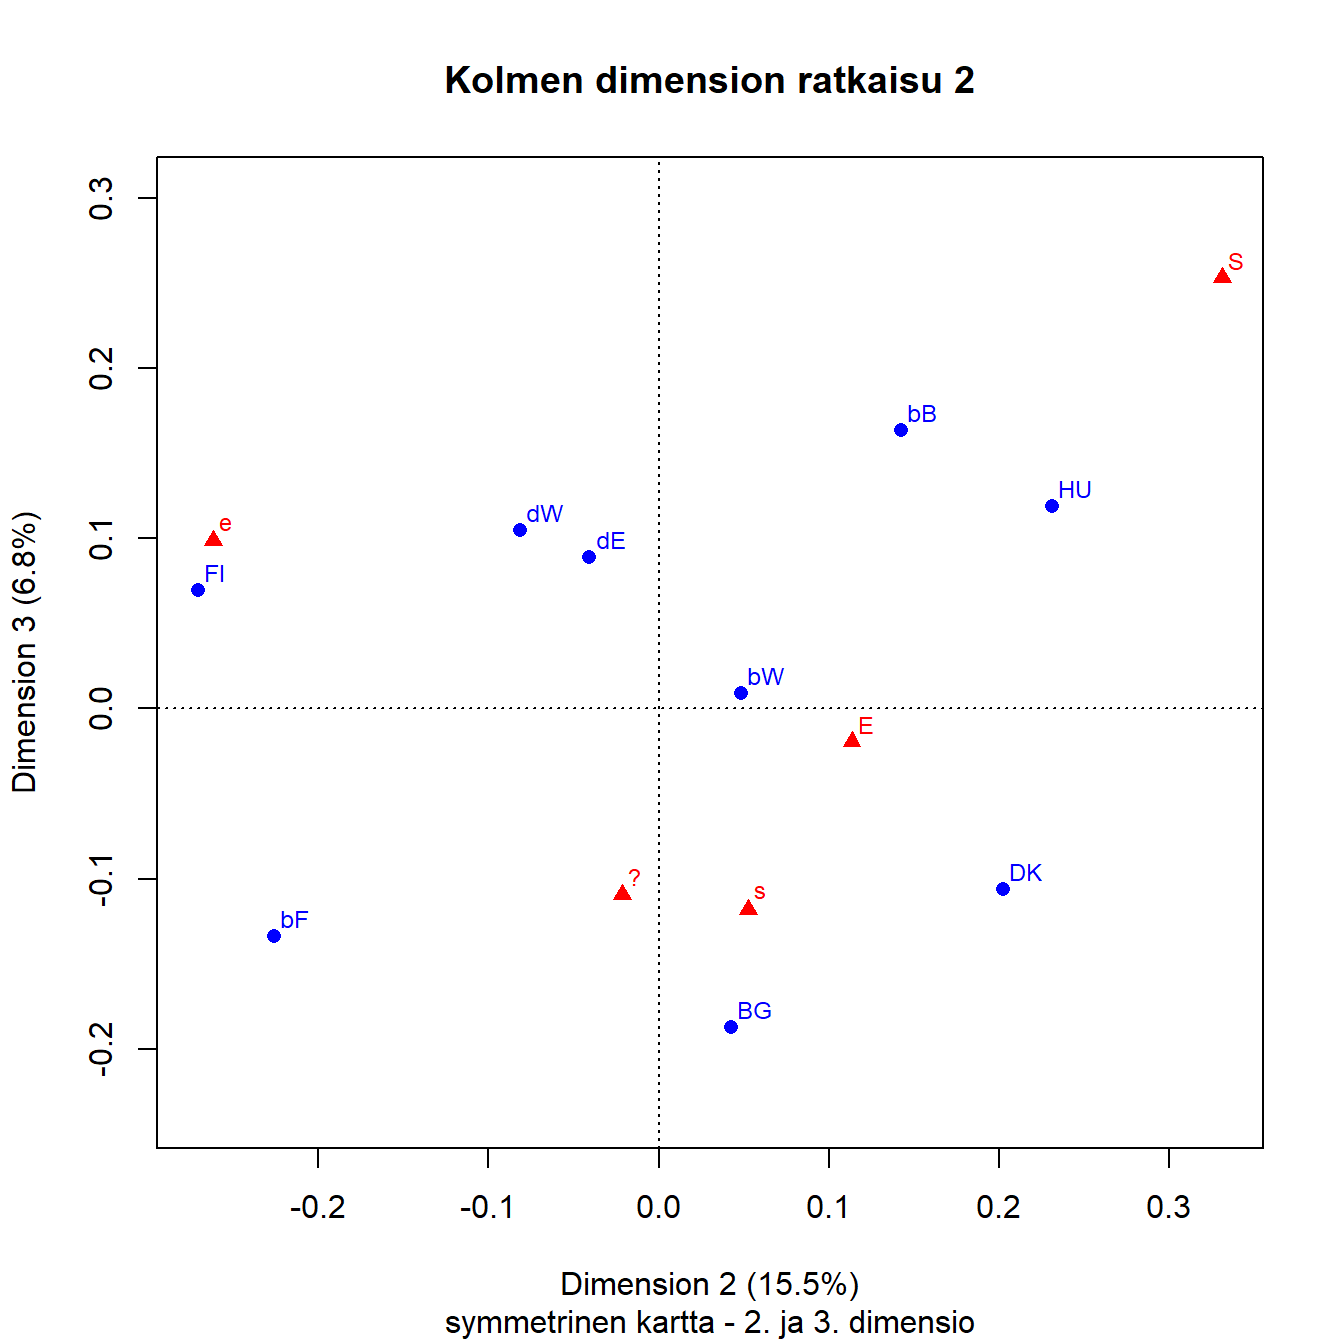
\includegraphics[width=0.9\linewidth]{JH_capaper_files/figure-latex/suppointCA3map3-1} 

}

\caption{Q1b: Saksan ja  Belgian aluejako }\label{fig:suppointCA3map3}
\end{figure}

\textbf{k} Tulkinta.

\textbf{k} kokeilu 3d-grafiikalla - toinen riittää

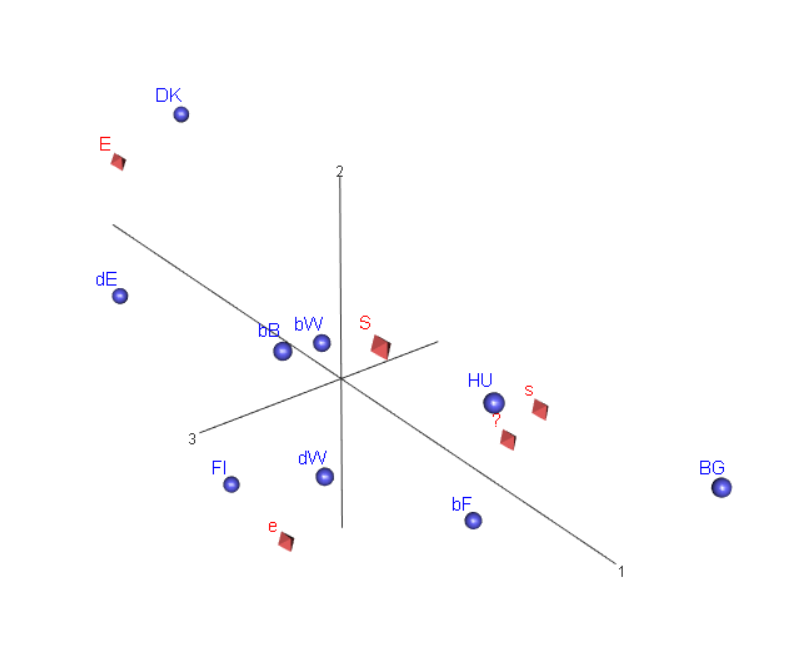
\includegraphics[width=11.07in]{img/3dSymMap_1}
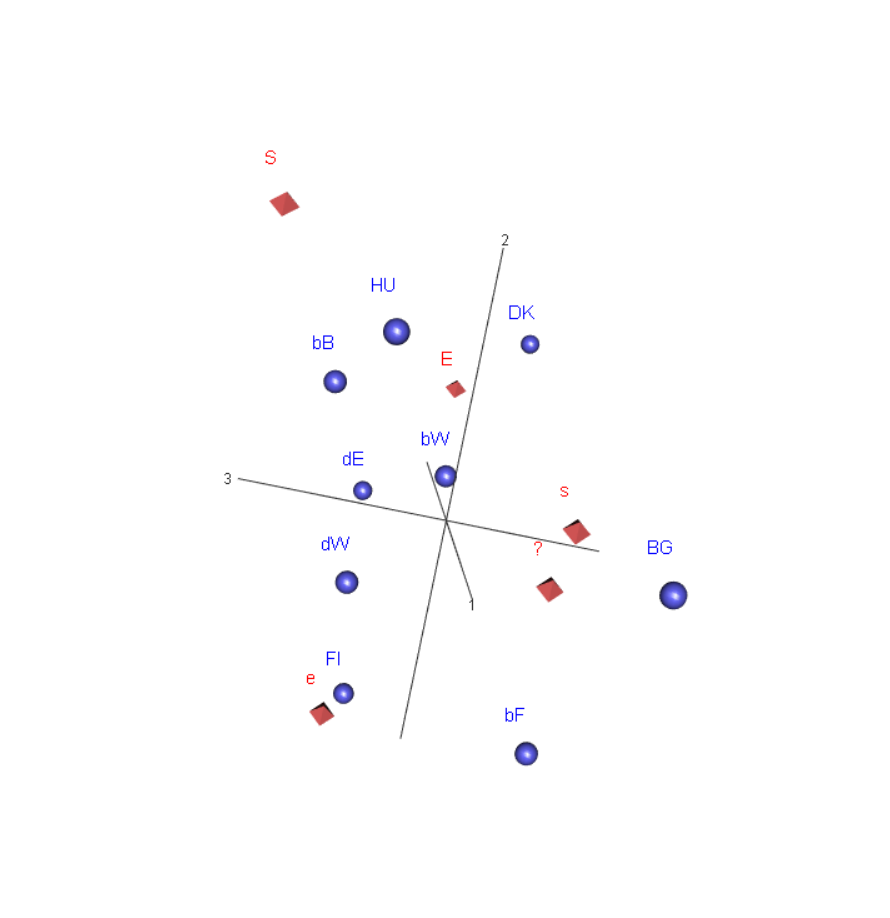
\includegraphics[width=12.36in]{img/3dSymMap_2}

  \bibliography{jhca2020.bib,packages.bib}

\end{document}
